\documentclass[lettersize,journal]{IEEEtran}

\usepackage{amsmath,amsfonts,amssymb,amsthm}
\usepackage{mathtools}
\usepackage{array}
\usepackage[caption=false,font=normalsize,labelfont=sf,textfont=sf]{subfig}
\usepackage{textcomp}
\usepackage{stfloats}
\usepackage{url}
\usepackage{graphicx}
\usepackage{cite}
\usepackage{booktabs}
\usepackage{multirow}
\usepackage{tikz}
\usetikzlibrary{arrows.meta,shapes.geometric,positioning,fit,backgrounds}

\hyphenation{op-tical net-works semi-conduc-tor IEEE-Xplore auto-en-coder auto-en-coders vari-a-tional}

%% Notation shortcuts
\newcommand{\dID}{d_{\mathrm{ID}}}
\newcommand{\dz}{m}
\newcommand{\dzopt}{m^*}
\newcommand{\dtrue}{d_{\mathrm{true}}}
\newcommand{\Jg}{J_g}
\newcommand{\R}{\mathbb{R}}
\newcommand{\kap}{\kappa}
\newcommand{\AUsat}{\mathrm{AU}_{\mathrm{sat}}}
\newcommand{\dzsat}{m^{\mathrm{sat}}}
\newcommand{\mknee}{m^{\mathrm{knee}}}
\newcommand{\demb}{d_{\mathrm{emb}}}

\newtheorem{theorem}{Theorem}
\newtheorem{proposition}{Proposition}
\newtheorem{definition}{Definition}
\newtheorem{remark}{Remark}

\begin{document}

\title{Intrinsic Dimension Estimation as a Design Principle for Autoencoder Bottleneck Dimensions}

\author{Anonymous~Author
\thanks{Manuscript submitted for review.}}

\markboth{IEEE Transactions on Neural Networks and Learning Systems}%
{Author: Intrinsic Dimension Estimation for AE Bottleneck Design}

\maketitle

\begin{abstract}
Selecting the bottleneck dimension $m$ of an autoencoder (AE) has traditionally relied on expensive manual sweeps or empirical heuristics, leaving the design rationale unclear.
This paper proposes a two-stage pipeline that uses intrinsic dimension (ID) estimation as a principled guide for bottleneck design:
(1) estimate the intrinsic dimension $\hat{d}_\mathrm{ID}$ via TwoNN/MLE to narrow the search range, and
(2) identify the optimal bottleneck dimension $m^*$ using the active units (AU) pattern of a variational autoencoder (VAE)---adopting the saturation dimension $m^\mathrm{sat}$ for manifolds with sharp saturation, or the AU inflection point $m^\mathrm{knee}$ for gradually increasing datasets---with CKA and MSE elbow as auxiliary criteria.
Experiments on synthetic manifolds (Swiss Roll, Torus, M\"{o}bius Band) and MNIST yield three main findings:
\textbf{(RQ1)} $\hat{d}_\mathrm{ID}$ serves as a strong prior indicator, aligning well with $m^*$ especially on synthetic manifolds (with limited accuracy on real data);
\textbf{(RQ2)} For topologically nontrivial manifolds (Torus, M\"{o}bius Band), the VAE AU saturation value corresponds to the topological embedding dimension $d_\mathrm{emb}$ under standardized preprocessing;
\textbf{(RQ3)} Decoder Jacobian regularization (IsometricAE) achieves near-isometric embedding ($\kappa \approx 1$), realizing the prerequisite for reliable ID estimation in latent space.
A secondary finding quantifies the temporal separation of global and local structure formation during MNIST training.
\end{abstract}

\begin{IEEEkeywords}
Autoencoder, bottleneck dimension, intrinsic dimension, variational autoencoder, active units, isometric embedding, manifold hypothesis, TwoNN, centered kernel alignment.
\end{IEEEkeywords}

%% ===================================================================
\section{Introduction}\label{sec:intro}
\IEEEPARstart{T}{he} manifold hypothesis~\cite{fefferman2016manifold,bengio2013representation} posits that high-dimensional natural data concentrate near a smooth low-dimensional manifold $\mathcal{M}$ (with $\dim\mathcal{M} = d \ll N$) embedded in $\R^N$.
Autoencoders (AEs) are implicitly designed to capture this manifold in latent space, yet the bottleneck dimension $m$ is typically chosen by manual validation sweeps---a computationally expensive process with no principled justification.

\subsection{Research Aim}

We propose to \emph{estimate the intrinsic dimension $\dID$ of the data in advance} and use it as a design guide for the bottleneck dimension.
We adopt TwoNN~\cite{facco2017twonn} and MLE~\cite{levina2005mle} as ID estimators and quantify their relationship to the optimal AE bottleneck dimension.

\textbf{Theoretical motivation.}
Two distinct mechanisms link $\dID$ and $m^*$:
\begin{itemize}
  \item \textbf{Why AEs need at least $\dID$ dimensions:}
    When data lie locally on a $\dID$-dimensional manifold, the bottleneck must satisfy $m \geq \dID$ to bound reconstruction error under standard smoothness assumptions (Theorem~\ref{thm:lower_bound}).
    Hence $\dID$ provides a principled \emph{lower-bound guideline} estimable before training.
  \item \textbf{Why VAE AU converges near $\demb$:}
    The support $\R^m$ of the Gaussian prior in a VAE is topologically contractible; embedding a manifold with nontrivial fundamental group $\pi_1$ (e.g., Torus with $\pi_1 = \mathbb{Z}^2$) without self-intersection requires $\demb > \dID$ dimensions~\cite{hatcher2002algebraic}.
    Under KL regularization, AU tends to converge near $\demb$ in sufficiently capable VAEs (Proposition~\ref{thm:au}).
\end{itemize}

\subsection{Two Notions of Dimension}\label{sec:intro_dim}

This paper employs two fundamentally different concepts of manifold dimension:

\textbf{Local Intrinsic Dimension $\dID$:}
The dimension of the tangent space at each point of $\mathcal{M}$---a local geometric quantity measuring the degrees of freedom in a neighborhood.
Both the Swiss Roll and the Torus have $\dID = 2$.
TwoNN and MLE estimate $\dID$ from local distance relations.

\textbf{Topological Embedding Dimension $\demb$:}
The minimum dimension of Euclidean space $\R^{\demb}$ into which $\mathcal{M}$ can be continuously embedded without self-intersection.
For simply connected manifolds ($\pi_1 = \{1\}$, e.g., Swiss Roll) $\demb = \dID$; for manifolds with nontrivial $\pi_1$ (e.g., Torus: $\pi_1 = \mathbb{Z}^2$) $\demb > \dID$~\cite{hatcher2002algebraic,guillemin1974differential}.

\textbf{Central claim:} AEs reflect $\dID$ (tangent-space dimension) through MSE minimization, while VAE AU saturation reflects $\demb$ (topological embedding dimension) via the continuous-mapping constraint.
These two findings coexist without logical contradiction.

\subsection{Research Questions}

\begin{description}
  \item[\textbf{RQ1}] Can TwoNN/MLE accurately estimate $\dtrue$ on synthetic manifolds, and does $\hat{\dID}$ align with $m^*$ to a degree useful for design guidance?
  \item[\textbf{RQ2}] To what extent does VAE $\AUsat$ reflect the topological properties (fundamental group $\pi_1$) of the manifold?
  \item[\textbf{RQ3}] Can isometric embedding be achieved by decoder Jacobian regularization, and how does this differ from encoder-side regularization (CAE)?
\end{description}

\subsection{Contributions}

\begin{enumerate}
  \item \textbf{Systematic evaluation of ID estimators (RQ1):}
    We benchmark TwoNN and MLE on synthetic manifolds and demonstrate that $\hat{\dID}$ serves as a strong prior for AE bottleneck design, particularly for synthetic data (Experiments E1--E3).
  \item \textbf{Observation of VAE $\AUsat$ on topologically nontrivial manifolds (RQ2):}
    On Torus and M\"{o}bius Band, VAE $\AUsat$ corresponds to the topological minimum embedding dimension under standardized preprocessing (Experiments EA, EB).
  \item \textbf{Isometric embedding via IsometricAE (RQ3):}
    Decoder Jacobian regularization achieves $\kap \approx 1$ (Experiment EC).
  \item \textbf{Temporal separation of global/local structure in MNIST (secondary finding):}
    We quantify how global neighborhood structure forms rapidly in early training while local ID increases gradually (Experiment E6).
\end{enumerate}

%% ===================================================================
\section{Related Work}\label{sec:related}

\subsection{Intrinsic Dimension Estimation}

TwoNN~\cite{facco2017twonn} estimates ID from the ratio $\mu_i = r_2/r_1$ of two nearest-neighbor distances, offering high accuracy and computational efficiency.
MLE~\cite{levina2005mle} constructs a maximum-likelihood estimator from $k$-nearest-neighbor distances, giving stable estimates across choices of $k$.
DANCo~\cite{ceruti2014danco} uses joint distributions of angles and distances for finer estimation at higher computational cost.
Pope et al.~\cite{pope2021intrinsic} showed that natural images have much lower ID than pixel dimension as measured by TwoNN.
More recent work has analyzed ID of deep network representations: Ansuini et al.~\cite{ansuini2019intrinsic} quantified layer-wise ID in deep networks; Birdal et al.~\cite{birdal2021intrinsic} studied the connection between ID, persistent homology, and generalization; Valeriani et al.~\cite{valeriani2023geometry} reported a ``hump'' structure of layer-wise ID in large transformer models.

A known limitation of TwoNN is its \emph{underestimation bias} near manifold boundaries and in high-curvature regions~\cite{facco2017twonn}.
ID estimates at $m = \dtrue$ (the boundary of the underfitting regime) are particularly susceptible to this bias.

\subsection{VAE Gaussian Prior and Topological Embedding}

The support of the standard Gaussian prior $\mathcal{N}(0, I_m)$ is topologically contractible (any loop can be continuously contracted to a point)~\cite{hatcher2002algebraic}.
Therefore, embedding a manifold with nontrivial $\pi_1$ (e.g., Torus $T^2$ with $\pi_1 = \mathbb{Z}^2$) without self-intersection requires at least $\demb > \dID$ dimensions~\cite{hatcher2002algebraic,guillemin1974differential}.
KL regularization thus tends to drive $\AUsat$ toward $\demb$ in sufficiently capable VAEs (Proposition~\ref{thm:au}, Experiments EA, EB).

\subsection{AE Bottleneck Dimension and Representation Quality}

$\beta$-VAE~\cite{higgins2017betavae} promotes disentangled representations by increasing the weight of KL regularization.
Lucas et al.~\cite{lucas2019elbo} analyzed posterior collapse conditions in linear VAEs and theoretically showed that AU saturates near $d_\mathrm{ID}$; however, their analysis assumes a single linear manifold and does not systematically examine topologically nontrivial cases ($\AUsat \approx \demb$).
Nazari et al.~\cite{nazari2023geometric} and Kato et al.~\cite{kato2020rdae} proposed isometric AEs via decoder Jacobian regularization.
Contractive AE (CAE)~\cite{rifai2011cae} penalizes the encoder Frobenius norm; denoising AE (DAE)~\cite{alain2014dae} implicitly estimates the score function and learns tangent-direction-selective representations.

\textbf{Distinction from prior work:}
Existing studies mostly evaluate AE performance with a single metric.
This paper constructs a multi-metric pipeline (ID estimation, AU, CKA, condition number $\kap$, Trustworthiness) and demonstrates $m^* \approx \hat{\dID}$ on both synthetic and real data, with explicit consideration of TwoNN's underestimation bias.

%% ===================================================================
\section{Proposed Framework}\label{sec:framework}

We denote the bottleneck dimension consistently as $m$ ($:= d_z$), the optimal bottleneck as $m^*$, and the AU saturation dimension as $m^\mathrm{sat}$.

\subsection{Notation Summary}

Table~\ref{tab:notation} summarizes the key symbols used throughout this paper.

\begin{table*}[!t]
\centering
\caption{Key Notation}
\label{tab:notation}
\small
\begin{tabular}{l p{8cm} l}
\toprule
Symbol & Meaning & Reference \\
\midrule
$m$ & AE bottleneck dimension (design parameter) & \S\ref{sec:framework} \\
$m^*$ & Optimal bottleneck dimension & \S\ref{sec:framework} \\
$m^\mathrm{sat}$ & Dimension at which AU first saturates (saturation-type) & Eq.~\eqref{eq:dzopt_sat} \\
$m^\mathrm{knee}$ & AU growth inflection point (gradual-type) & Eq.~\eqref{eq:dzopt_knee} \\
$\AUsat$ & Maximum active units reached on grid & Eq.~\eqref{eq:dzopt_sat} \\
$\mathrm{AU}(m)$ & Active unit count at bottleneck $m$ & \S\ref{sec:framework} \\
$\hat{\dID}$ & ID estimate from TwoNN/MLE & \S\ref{sec:framework} \\
$\dtrue$ & True ID of synthetic manifold (known) & \S\ref{sec:exp_synthetic} \\
$\demb$ & Topological minimum embedding dimension & \S\ref{sec:intro_dim} \\
$\kap$ & Condition number of decoder Jacobian (isometry metric) & \S\ref{sec:related} \\
$r(m)$ & Normalized AU growth rate & Eq.~\eqref{eq:au_rate} \\
$\tau_\mathrm{knee}$ & Inflection-point threshold (0.25 in this work) & Eq.~\eqref{eq:dzopt_knee} \\
\bottomrule
\end{tabular}
\end{table*}

\subsection{Two-Stage Pipeline}

The proposed framework consists of two stages.

\textbf{Stage~1: ID Estimator Evaluation and Selection.}
Benchmark TwoNN and MLE on synthetic manifolds with known $\dtrue$ to select a reliable estimator.
For real data with large input dimension $N$, apply TwoNN/MLE to the latent space of a reference AE trained with a large bottleneck ($m_\mathrm{ref} \gg \hat{\dID}$).

\textbf{Stage~2: Optimal Bottleneck Search via VAE Sweep.}
Sweep $m$ over a discrete grid
$\mathcal{M} = \{1, 2, 4, 8, 12, 16, 20, 32, 64, 128, 256\}$,
training a VAE ($\beta=4$) at each $m$ and computing $\mathrm{AU}(m)$.

\begin{remark}[Grid Resolution]\label{rem:grid_resolution}
Since $\mathcal{M}$ is an approximately log-scale grid, when $\dID$ falls between grid points (e.g., $\dID = 6$ between $m=4$ and $m=8$), the grid point where AU first exceeds $\dID$ serves as a conservative upper bound for $m^*$.
Practical recommendation: verify with a finer grid near $\hat{\dID}$.
\end{remark}

Fig.~\ref{fig:framework_flow} illustrates the proposed two-stage pipeline.

\begin{figure*}[!t]
\centering
\resizebox{\textwidth}{!}{%
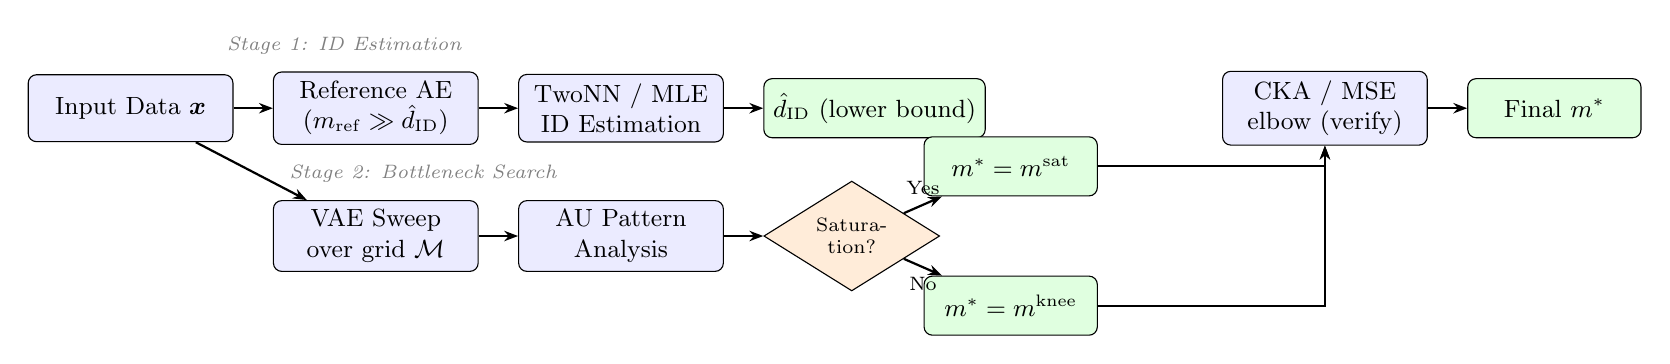
\begin{tikzpicture}[
  node distance=0.35cm and 0.5cm,
  box/.style={rectangle, draw, rounded corners=3pt, fill=blue!8, minimum height=0.85cm, minimum width=2.6cm, align=center, font=\small},
  decision/.style={diamond, draw, fill=orange!15, minimum height=0.8cm, minimum width=1.6cm, align=center, font=\scriptsize, aspect=1.6},
  result/.style={rectangle, draw, rounded corners=3pt, fill=green!12, minimum height=0.75cm, minimum width=2.2cm, align=center, font=\small},
  arrow/.style={-{Stealth[length=5pt]}, thick},
  label/.style={font=\scriptsize\itshape, text=gray}
]
%% Stage 1
\node[box] (data)   {Input Data $\boldsymbol{x}$};
\node[box, right=of data] (refAE) {Reference AE\\($m_\mathrm{ref} \gg \hat{d}_\mathrm{ID}$)};
\node[box, right=of refAE] (idest) {TwoNN / MLE\\ID Estimation};
\node[result, right=of idest] (hatd) {$\hat{d}_\mathrm{ID}$ (lower bound)};

%% Stage 2
\node[box, below=0.7cm of refAE] (vaesw) {VAE Sweep\\over grid $\mathcal{M}$};
\node[box, right=of vaesw] (aupat) {AU Pattern\\Analysis};
\node[decision, right=of aupat] (branch) {Satura-\\tion?};
\node[result, above right=0.15cm and 0.35cm of branch] (sat) {$m^* = m^\mathrm{sat}$};
\node[result, below right=0.15cm and 0.35cm of branch] (knee) {$m^* = m^\mathrm{knee}$};

%% Aux
\node[box, right=3.0cm of hatd] (aux) {CKA / MSE\\elbow (verify)};
\node[result, right=of aux] (mstar) {Final $m^*$};

%% Arrows Stage 1
\draw[arrow] (data) -- (refAE);
\draw[arrow] (refAE) -- (idest);
\draw[arrow] (idest) -- (hatd);

%% Arrows Stage 2
\draw[arrow] (data) -- (vaesw);
\draw[arrow] (vaesw) -- (aupat);
\draw[arrow] (aupat) -- (branch);
\draw[arrow] (branch) -- node[above, font=\scriptsize]{Yes} (sat);
\draw[arrow] (branch) -- node[below, font=\scriptsize]{No} (knee);
\draw[arrow] (sat) -| (aux);
\draw[arrow] (knee) -| (aux);
\draw[arrow] (aux) -- (mstar);

%% Labels
\node[label, above=0.1cm of refAE, xshift=-0.4cm] {Stage 1: ID Estimation};
\node[label, above=0.1cm of vaesw, xshift=0.6cm] {Stage 2: Bottleneck Search};
\end{tikzpicture}%
}% end resizebox
\caption{Proposed two-stage pipeline for bottleneck dimension design. Stage~1 trains a reference AE to estimate $\hat{d}_\mathrm{ID}$ via TwoNN/MLE. Stage~2 sweeps a VAE over a grid, classifies the AU pattern as saturation-type or gradual-type, and selects $m^*$ using CKA and MSE as auxiliary criteria.}
\label{fig:framework_flow}
\end{figure*}

\subsection{Optimal Bottleneck Dimension}

The normalized AU growth rate is defined as
\begin{equation}
  r(m) = \frac{\mathrm{AU}(m) - \mathrm{AU}(m_\mathrm{prev})}{m - m_\mathrm{prev}}
  \label{eq:au_rate}
\end{equation}
where $m_\mathrm{prev}$ is the preceding grid point in $\mathcal{M}$.

\textbf{AU Pattern Classification:}
\begin{itemize}
  \item \textbf{Saturation-type:} AU maintains the same value at two or more consecutive grid points (plateau width $\geq 2$). Typical examples: Swiss Roll, Torus.
  \item \textbf{Gradual-type:} AU increases nearly monotonically across the entire grid; $\mathrm{AU}(m_{\max}) \approx \AUsat$ is reached only at the largest $m$. Typical example: MNIST.
\end{itemize}

\textbf{Case-based definition of $m^*$:}
\begin{equation}
  m^* =
  \begin{cases}
    m^\mathrm{sat} \coloneqq \min\{m \in \mathcal{M} \mid \mathrm{AU}(m) = \AUsat\} \\
      \quad\text{(saturation-type)} \\[4pt]
    m^\mathrm{knee} \coloneqq \min\{m \in \mathcal{M} \mid r(m) < \tau_\mathrm{knee} \cdot r_\mathrm{max}\} \\
      \quad\text{(gradual-type)}
  \end{cases}
  \label{eq:dzopt}
\end{equation}
where
\begin{align}
  \AUsat &= \max_{m' \in \mathcal{M}} \mathrm{AU}(m'), \label{eq:dzopt_sat} \\
  r_\mathrm{max} &= \max_{m' \in \mathcal{M}} r(m'), \quad \tau_\mathrm{knee} = 0.25. \label{eq:dzopt_knee}
\end{align}

\textbf{Design Rule (two-branch):}

\noindent\underline{Saturation-type}: Given the saturation set $\mathcal{C}_\mathrm{sat} = \{m \in \mathcal{M} \mid \mathrm{AU}(m) = \AUsat\}$,
\begin{multline}
  m^* = \min\!\Bigl\{m \in \mathcal{C}_\mathrm{sat} \;\Big|\; \\
  \mathrm{CKA}(m) \geq (1-\varepsilon)\max_{m'\in\mathcal{C}_\mathrm{sat}}\mathrm{CKA}(m')
  \Bigr\}
  \label{eq:dzopt_cka}
\end{multline}
with $\varepsilon = 0.01$. Verify consistency with the MSE elbow $m^*_\mathrm{elbow}$ (Eq.~\eqref{eq:elbow_def}).

\noindent\underline{Gradual-type}: Given $\mathcal{C}_\mathrm{knee} = \{m \in \mathcal{M} \mid m \geq m^\mathrm{knee},\; r(m) < \tau_\mathrm{knee} \cdot r_\mathrm{max}\}$,
\begin{multline}
  m^* = \min\!\Bigl\{m \in \mathcal{C}_\mathrm{knee} \;\Big|\; \\
  \mathrm{CKA}(m) \geq (1-\varepsilon)\max_{m'\in\mathcal{C}_\mathrm{knee}}\mathrm{CKA}(m')
  \Bigr\}
  \label{eq:dzopt_cka_knee}
\end{multline}

\textbf{Rationale for AU as primary criterion:}
Unlike AIC/BIC, which require an effective parameter count (ill-defined for nonlinear AEs), AU saturation directly measures the \emph{information dimensions actually used} by the model under KL regularization, providing a data-driven model selection criterion independent of AIC/BIC (see Proposition~\ref{thm:au}).

\subsection{Evaluation Metrics}

\textbf{TwoNN ID estimator}~\cite{facco2017twonn}: Uses the ratio $\mu_i = r_2/r_1$ of the two nearest-neighbor distances,
\begin{equation}
  \hat{\dID}^\mathrm{TwoNN} = \frac{1}{\mathbb{E}[\log \mu_i]}.
\end{equation}

\textbf{MLE ID estimator}~\cite{levina2005mle}: Maximum-likelihood estimate from $k$-nearest-neighbor distance ratios,
\begin{equation}
  \hat{\dID}^\mathrm{MLE} = \left[\frac{1}{k-1}\sum_{j=1}^{k-1}\log\frac{r_k(\boldsymbol{x}_i)}{r_j(\boldsymbol{x}_i)}\right]^{-1}.
\end{equation}

\textbf{Active Units (AU)}~\cite{lucas2019elbo}: A latent dimension $k$ is active if
$V_k = \mathrm{Var}_{\boldsymbol{x}}[\mathbb{E}_{q_\phi}[z_k|\boldsymbol{x}]] > \delta$,
\begin{equation}
  \mathrm{AU} = \sum_{k=1}^{m} \mathbf{1}[V_k > \delta], \quad \delta = 10^{-2}.
  \label{eq:au}
\end{equation}

\textbf{CKA}~\cite{kornblith2019cka}: Given input $\boldsymbol{X}$ and reconstruction $\hat{\boldsymbol{X}}$, with kernel matrices $K = \boldsymbol{X}\boldsymbol{X}^\top$, $L = \hat{\boldsymbol{X}}\hat{\boldsymbol{X}}^\top$, and centering matrix $H = I_n - \frac{1}{n}\boldsymbol{1}\boldsymbol{1}^\top$,
\begin{equation}
  \mathrm{CKA}(K, L) = \frac{\mathrm{HSIC}(K, L)}{\sqrt{\mathrm{HSIC}(K,K)\cdot\mathrm{HSIC}(L,L)}}
  \label{eq:cka}
\end{equation}
where $\mathrm{HSIC}(K,L) = \frac{1}{(n-1)^2}\mathrm{tr}(KHLH)$.

\textbf{Condition number $\kap$}: Ratio of largest to smallest singular values of decoder Jacobian $\Jg(z) \in \R^{N\times m}$,
$\kap = \sigma_1/\sigma_m$.

\textbf{MSE elbow}: After smoothing $\tilde{\mathcal{L}}(m_k) = \frac{1}{2w+1}\sum_{j=-w}^{w}\mathcal{L}(m_{k+j})$ (window $w=1$), we compute normalized second differences
\begin{equation}
  \Delta^2(m_k) = \frac{\tilde{\mathcal{L}}(m_{k-1}) - 2\tilde{\mathcal{L}}(m_k) + \tilde{\mathcal{L}}(m_{k+1})}{\tilde{\mathcal{L}}(m_1)},
  \label{eq:elbow}
\end{equation}
\begin{equation}
  m^*_\mathrm{elbow} = \arg\max_{k \in \{2,\ldots,K-1\}} \Delta^2(m_k).
  \label{eq:elbow_def}
\end{equation}

%% ===================================================================
\section{Theoretical Background}\label{sec:theory}

The following theorems and propositions provide the theoretical interpretation of our experiments.
Proofs are included for all results.

\begin{theorem}[Bottleneck Lower Bound]\label{thm:lower_bound}
For a data distribution $p(\boldsymbol{x})$ concentrated on a smooth $d$-dimensional manifold $\mathcal{M} \subset \R^N$, having bounded expected reconstruction error requires $m \geq d$.
\end{theorem}

\begin{proof}
Consider an AE with encoder $f: \R^N \to \R^m$ and decoder $g: \R^m \to \R^N$.
Assume $m < d$.
Since $f$ is continuous, the image of the composition $g \circ f: \R^N \to \R^N$ is contained in $g(\R^m)$, a set of dimension at most $m$.
Since $\mathcal{M}$ is a smooth $d$-dimensional manifold with $d > m$, by Sard's theorem the intersection of $\mathcal{M}$ with any set of dimension $\leq m$ has $\mathcal{M}$-measure zero.
Therefore $g(f(\boldsymbol{x})) = \boldsymbol{x}$ cannot hold $p$-almost everywhere, so
$\mathbb{E}_{p}[\|\boldsymbol{x} - g(f(\boldsymbol{x}))\|^2] > 0$ cannot be made to vanish.
Hence $m \geq d$ is necessary.
\end{proof}

Experiment E1 (Swiss Roll, $\dtrue = 2$) confirms this: MSE drops approximately 35-fold ($1.016 \to 0.029$, 3-seed average) at the $m=1 \to 2$ transition.

\begin{proposition}[Effective Rank of Decoder Jacobian]\label{thm:rank}
When a sufficiently capable AE achieves accurate reconstruction of $\mathcal{M}$, the number of significant singular values of $\Jg(z) \in \R^{N\times m}$ equals $r^* = \min(m, \demb)$.
For $m \leq \demb$: $\mathrm{rank}\,\Jg(z) = m$; for $m > \demb$: surplus dimensions degenerate and $\mathrm{rank}\,\Jg(z) = \demb$.
\end{proposition}

\begin{proof}
When the AE accurately encodes $\mathcal{M}$, the image of $g$ locally covers a neighborhood of $\mathcal{M}$.
The image of the differential $\Jg(z): \R^m \to \R^N$ spans the tangent space $T_{g(z)}\mathcal{M}$.
Since $\mathcal{M}$ is $d$-dimensional, $\dim T_{g(z)}\mathcal{M} = d$, so $\mathrm{rank}(\Jg(z)) = \min(m, d)$.
When $m > d$, the $m - d$ surplus directions in $\R^m$ have no corresponding tangent-space components;
gradient-based training drives their singular values toward zero.
\end{proof}

Experiment E2 confirms: for $m > \demb$ (Torus, $m=4$, $\demb=3$), the significant singular value count is 3.00.

\begin{theorem}[Pullback Metric and Isometry]\label{thm:pullback}
When decoder $g: \R^m \to \R^N$ is an isometric embedding into the Riemannian manifold $(\mathcal{M}, g_\mathcal{M})$, the pullback metric $G(z) = \Jg(z)^\top \Jg(z)$ is proportional to the identity, i.e., $\kap = 1$.
\end{theorem}

\begin{proof}
By definition of an isometric embedding, for any $z \in \R^m$ and tangent vectors $u, v \in \R^m$:
$(g_\mathcal{M})_{g(z)}(\Jg(z)u,\, \Jg(z)v) = u^\top v$.
The pullback metric satisfies $(g^* g_\mathcal{M})_z(u,v) = u^\top G(z)\, v$, where $G(z) = \Jg(z)^\top \Jg(z)$.
Isometry therefore implies $u^\top G(z) v = u^\top v$ for all $u, v$, so $G(z) = I_m$.
Hence all singular values of $\Jg(z)$ are equal to 1, giving $\kap = \sigma_{\max}/\sigma_{\min} = 1$.
\end{proof}

Experiment EC shows IsometricAE achieves $\kap \approx 1.055$.

\begin{proposition}[Noise Selectivity]\label{thm:nsr}
The optimal denoising AE approximates the score function $\nabla_{\boldsymbol{x}}\log p(\boldsymbol{x})$.
An AE trained with $m = \dtrue$ selectively removes noise in the normal direction more than in the tangent direction.
\end{proposition}

\begin{proof}
By the result of Alain and Bengio~\cite{alain2014dae}, the reconstruction residual of a denoising AE satisfies
$r(\boldsymbol{x}) - \boldsymbol{x} \approx \sigma^2 \nabla_{\boldsymbol{x}}\log p(\boldsymbol{x})$.
Under the manifold hypothesis, data density $p(\boldsymbol{x})$ decays sharply in normal directions and varies slowly along tangent directions.
Hence $\nabla_{\boldsymbol{x}}\log p(\boldsymbol{x})$ points predominantly in the normal direction,
and the reconstruction correction selectively suppresses normal-direction noise.
\end{proof}

Experiment E3 confirms: at $m = \dtrue$, normal-direction error $>$ tangent-direction error.

\begin{proposition}[KL Regularization Required for AU Saturation]\label{thm:au}
For a Vanilla AE (no regularization), $\mathrm{AU} = m$ for any $m > \dID$.
AU saturation at $\dID$ requires KL regularization (the information bottleneck constraint).
\end{proposition}

\begin{proof}
The VAE objective is $\mathcal{L} = \mathcal{L}_{\mathrm{rec}} + \beta D_{\mathrm{KL}}(q(z|\boldsymbol{x})\|p(z))$.
For dimensions beyond the intrinsic dimension of the data, the encoder posterior $q(z_k|\boldsymbol{x})$ carries no information
about $\boldsymbol{x}$; the KL term forces $q(z_k|\boldsymbol{x}) \to p(z_k) = \mathcal{N}(0,1)$, eliminating the information channel.
Consequently, the variance $\mathrm{Var}_{\boldsymbol{x}}[\mathbb{E}_q[z_k|\boldsymbol{x}]]$ collapses below the threshold $\delta = 10^{-2}$,
deactivating those units.
A Vanilla AE has no such penalty, so all $m$ dimensions remain active ($\mathrm{AU} = m$) regardless of the data dimensionality.
\end{proof}

Experiment EA confirms: only VAE ($\beta=4$) exhibits AU saturation; Vanilla AE always has $\mathrm{AU} = m$.

\begin{proposition}[Neighborhood Preservation and Optimal Bottleneck]\label{thm:trust}
At $m = \dtrue$ (or the topological minimum embedding dimension), Trustworthiness improves sharply, and further increases in $m$ yield limited additional improvement.
\end{proposition}

\begin{proof}
By Theorem~\ref{thm:lower_bound}, for $m < d$ the encoder $f$ cannot be injective on $\mathcal{M}$, causing
unavoidable ``information collisions'' that distort local neighborhoods, reducing Trustworthiness.
At $m \geq d$, the topological obstruction is removed: a homeomorphic (structure-preserving) mapping can be learned,
and Trustworthiness improves sharply.
For $m > d$, the additional dimensions provide negligible benefit as the neighborhood structure is already well-preserved.
\end{proof}

Experiment E5 confirms: Swiss Roll ($\Delta \approx 0.015$ at $m=2$) and Torus ($\Delta \approx 0.015$ at $m=3=\demb$).

Table~\ref{tab:theorem_exp} summarizes the theorem-experiment correspondences.

\begin{table*}[!t]
\centering
\caption{Theorem--Experiment Correspondence}
\label{tab:theorem_exp}
\begin{tabular}{l p{7cm} l}
\toprule
Theorem & Claim & Experiment \\
\midrule
Thm.~\ref{thm:lower_bound} (lower bound) & MSE spikes for $m < \dtrue$ & E1 \\
Prop.~\ref{thm:rank} (effective rank) & Significant singular values $= m$ & E2 \\
Thm.~\ref{thm:pullback} (pullback metric) & $\kap \approx 1$ isometry & EC \\
Prop.~\ref{thm:nsr} (noise selectivity) & Normal direction selectively removed & E3 \\
Prop.~\ref{thm:au} (AU saturation) & KL regularization required & EA \\
Prop.~\ref{thm:trust} (neighborhood preservation) & Trustworthiness jumps at $m = \dtrue$ (or $\demb$) & E5 \\
Topological embedding (supplementary) & $\AUsat \approx \demb$ (conditional) & EB \\
\bottomrule
\end{tabular}
\end{table*}

%% ===================================================================
\section{Experiments}\label{sec:exp}

\subsection{Experimental Setup}\label{sec:exp_setup}

Common hyperparameters are listed in Table~\ref{tab:common_hp}; model-specific hyperparameters in Tables~\ref{tab:synthetic_hp} and~\ref{tab:mnist_hp}.

\begin{table}[!t]
\centering
\caption{Common Hyperparameters}
\label{tab:common_hp}
\begin{tabular}{ll}
\toprule
Parameter & Value \\
\midrule
Optimizer & Adam ($\mathrm{lr} = 1\times10^{-3}$) \\
Batch size & 128 \\
Activation & ReLU (output layer: Sigmoid) \\
Random seed & 42 (fixed) \\
Framework & PyTorch 2.0 \\
\bottomrule
\end{tabular}
\end{table}

\begin{table}[!t]
\centering
\caption{Synthetic Manifold AE/VAE Hyperparameters}
\label{tab:synthetic_hp}
\begin{tabular}{ll}
\toprule
Parameter & Value \\
\midrule
Hidden dims & $[64, 32]$ \\
Training epochs & 200--300 \\
VAE $\beta$ & 4.0 \\
IsometricAE $\lambda_\mathrm{iso}$ & 0.01 \\
Sample size & 5{,}000 (train 4{,}000 + test 1{,}000) \\
\bottomrule
\end{tabular}
\end{table}

\begin{table}[!t]
\centering
\caption{MNIST AE/VAE Hyperparameters}
\label{tab:mnist_hp}
\begin{tabular}{ll}
\toprule
Parameter & Value \\
\midrule
Input dim & 784 ($28\times28$ flattened) \\
Hidden dims & $[512, 256]$ \\
Training epochs & 300 (E4), 200 (E6) \\
VAE $\beta$ & 4.0 \\
Bottleneck $m$ & 1, 2, 4, 8, 12, 16, 20, 32, 64, 128, 256 \\
Batch size & 128 \\
\bottomrule
\end{tabular}
\end{table}

ID estimation uses $k=2$ for TwoNN and $k=10$ for MLE.
The AU threshold $\delta = 10^{-2}$ follows the standard value of~\cite{lucas2019elbo}.
Table~\ref{tab:rq_exp_map} lists the correspondence between experiments and research questions.

\begin{table*}[!t]
\centering
\caption{Research Questions and Experiment Mapping}
\label{tab:rq_exp_map}
\begin{tabular}{l l l p{6cm}}
\toprule
Exp. & RQ & Section & Purpose \\
\midrule
E1 & \textbf{RQ1} & \S\ref{sec:exp_synthetic} & ID estimation accuracy; $m^* \approx \hat{\dID}$ \\
E2 & Prop.~\ref{thm:rank}, Thm.~\ref{thm:pullback} basis & \S\ref{sec:exp_synthetic} & Decoder Jacobian rank and $\kap$ \\
E3 & Prop.~\ref{thm:nsr} & \S\ref{sec:exp_synthetic} & Noise selectivity (DAE) \\
E5 & Prop.~\ref{thm:trust} & \S\ref{sec:exp_e5} & Trustworthiness vs.\ $m$ \\
EA & \textbf{RQ2} & \S\ref{sec:exp_topology} & VAE AU saturation via KL regularization \\
EB & \textbf{RQ2} (depth) & \S\ref{sec:exp_topology} & $\AUsat$ vs.\ topological embedding dim. \\
EC & \textbf{RQ3} & \S\ref{sec:exp_topology} & Isometric embedding achievability \\
E4 & \textbf{RQ1} (real data) & \S\ref{sec:exp_mnist} & MNIST $m^* \approx \hat{\dID}$ \\
E6 & Novel finding & \S\ref{sec:exp_mnist} & MNIST training dynamics \\
EX & Statistical reliability & \S\ref{sec:exp_mnist} & Multi-seed stability \\
\bottomrule
\end{tabular}
\end{table*}

\textbf{AU threshold sensitivity analysis:}
We compared AU counts across $\delta \in \{0.001, 0.01, 0.05, 0.1\}$ for Swiss Roll and Torus VAE ($\beta=4$).
As shown in Table~\ref{tab:delta_sensitivity}, AU saturation values are \emph{completely robust} to the choice of $\delta$: Swiss Roll maintains AU$=2$ and Torus (at $m\geq6$) maintains AU$=3$ across all $\delta$ values.
This robustness arises because active dimensions have variance $O(1)$ while inactive dimensions have variance $O(10^{-4})$ or smaller, giving a two-order-of-magnitude gap that is insensitive to threshold changes.

\begin{table*}[!t]
\centering
\caption{AU Threshold Sensitivity (VAE $\beta=4$): AU values are completely robust to threshold choice}
\label{tab:delta_sensitivity}
\begin{tabular}{rcccc|cccc}
\toprule
 & \multicolumn{4}{c|}{Swiss Roll} & \multicolumn{4}{c}{Torus} \\
$m$ & $\delta{=}0.001$ & $\delta{=}0.01$ & $\delta{=}0.05$ & $\delta{=}0.1$
    & $\delta{=}0.001$ & $\delta{=}0.01$ & $\delta{=}0.05$ & $\delta{=}0.1$ \\
\midrule
2  & 2 & 2 & 2 & 2 & 2 & 2 & 2 & 2 \\
3  & 2 & 2 & 2 & 2 & 2 & 2 & 2 & 2 \\
6  & 2 & 2 & 2 & 2 & 3 & 3 & 3 & 3 \\
12 & 2 & 2 & 2 & 2 & 3 & 3 & 3 & 3 \\
16 & 2 & 2 & 2 & 2 & 3 & 3 & 3 & 3 \\
\bottomrule
\end{tabular}
\end{table*}

\subsection{ID Estimation and Optimal Bottleneck on Synthetic Manifolds (RQ1)}\label{sec:exp_synthetic}

\textbf{Question answered (RQ1):} Does TwoNN/MLE estimate $\dtrue$ accurately, and does $\hat{\dID}$ align with $m^*$ as a design guideline?

\subsubsection{Reconstruction Error Elbow Analysis (Experiment E1)}

We swept $m$ for Swiss Roll ($\dtrue = 2$, ambient $= 3$) and Torus ($\dtrue = 2$, ambient $= 3$), training AEs and recording MSE, AU, TwoNN ID, and MLE ID (3-seed mean $\pm$ std).
Results are shown in Tables~\ref{tab:e1_swissroll} and~\ref{tab:e1_torus}.

\begin{table}[!t]
\centering
\caption{E1: Swiss Roll ($\dtrue = 2$), 3-seed mean $\pm$ std}
\label{tab:e1_swissroll}
\begin{tabular}{rcccc}
\toprule
$m$ & MSE & AU & TwoNN ID & MLE ID \\
\midrule
1 & $1.0160\pm0.3150$ & $1.0\pm0.0$ & $1.00\pm0.00$ & $1.18\pm0.02$ \\
\textbf{2} & $\boldsymbol{0.0290\pm0.0010}$ & $2.0\pm0.0$ & $1.15\pm0.05$ & $1.12\pm0.00$ \\
3 & $0.0010\pm0.0000$ & $3.0\pm0.0$ & $1.94\pm0.06$ & $2.09\pm0.02$ \\
4 & $0.0010\pm0.0000$ & $4.0\pm0.0$ & $1.95\pm0.06$ & $2.10\pm0.01$ \\
\bottomrule
\end{tabular}
\end{table}

\begin{table}[!t]
\centering
\caption{E1: Torus ($\dtrue = 2$), 3-seed mean $\pm$ std. Bold row ($m=3$) is the effective elbow.}
\label{tab:e1_torus}
\small
\begin{tabular}{rcccc}
\toprule
$m$ & MSE & AU & TwoNN ID & MLE ID \\
\midrule
1           & $0.36\pm0.02$              & $1.00\pm0.00$ & $1.01\pm0.01$ & $1.12\pm0.00$ \\
2           & $0.11\pm0.01$              & $2.00\pm0.00$ & $1.86\pm0.04$ & $2.11\pm0.02$ \\
\textbf{3}  & $\boldsymbol{0.00\pm0.00}$ & $3.00\pm0.00$ & $2.02\pm0.00$ & $2.27\pm0.03$ \\
4           & $0.00\pm0.00$              & $4.00\pm0.00$ & $2.00\pm0.03$ & $2.28\pm0.02$ \\
\bottomrule
\end{tabular}
\end{table}

For Swiss Roll, MSE drops approximately 34-fold ($1.016 \to 0.029$) at $m = 2 = \dtrue$, confirming Theorem~\ref{thm:lower_bound}.
The standard deviation across 3 seeds is $\pm0.001$, demonstrating high robustness.
TwoNN ID at $m=2$ ($1.15\pm0.05$) underestimates the true ID of 2; this is the known finite-sample boundary bias~\cite{facco2017twonn}.
At $m=3$, TwoNN ID converges to $1.94\pm0.06$ and MLE to $2.09\pm0.02$, consistent with each other.

For Torus, the effective MSE elbow appears at $m=3$ despite $\dtrue=2$.
The topological explanation is discussed in \S\ref{sec:discussion_topology}.

Fig.~\ref{fig:e1_mse} shows the MSE elbow curves.

\begin{figure}[!t]
\centering
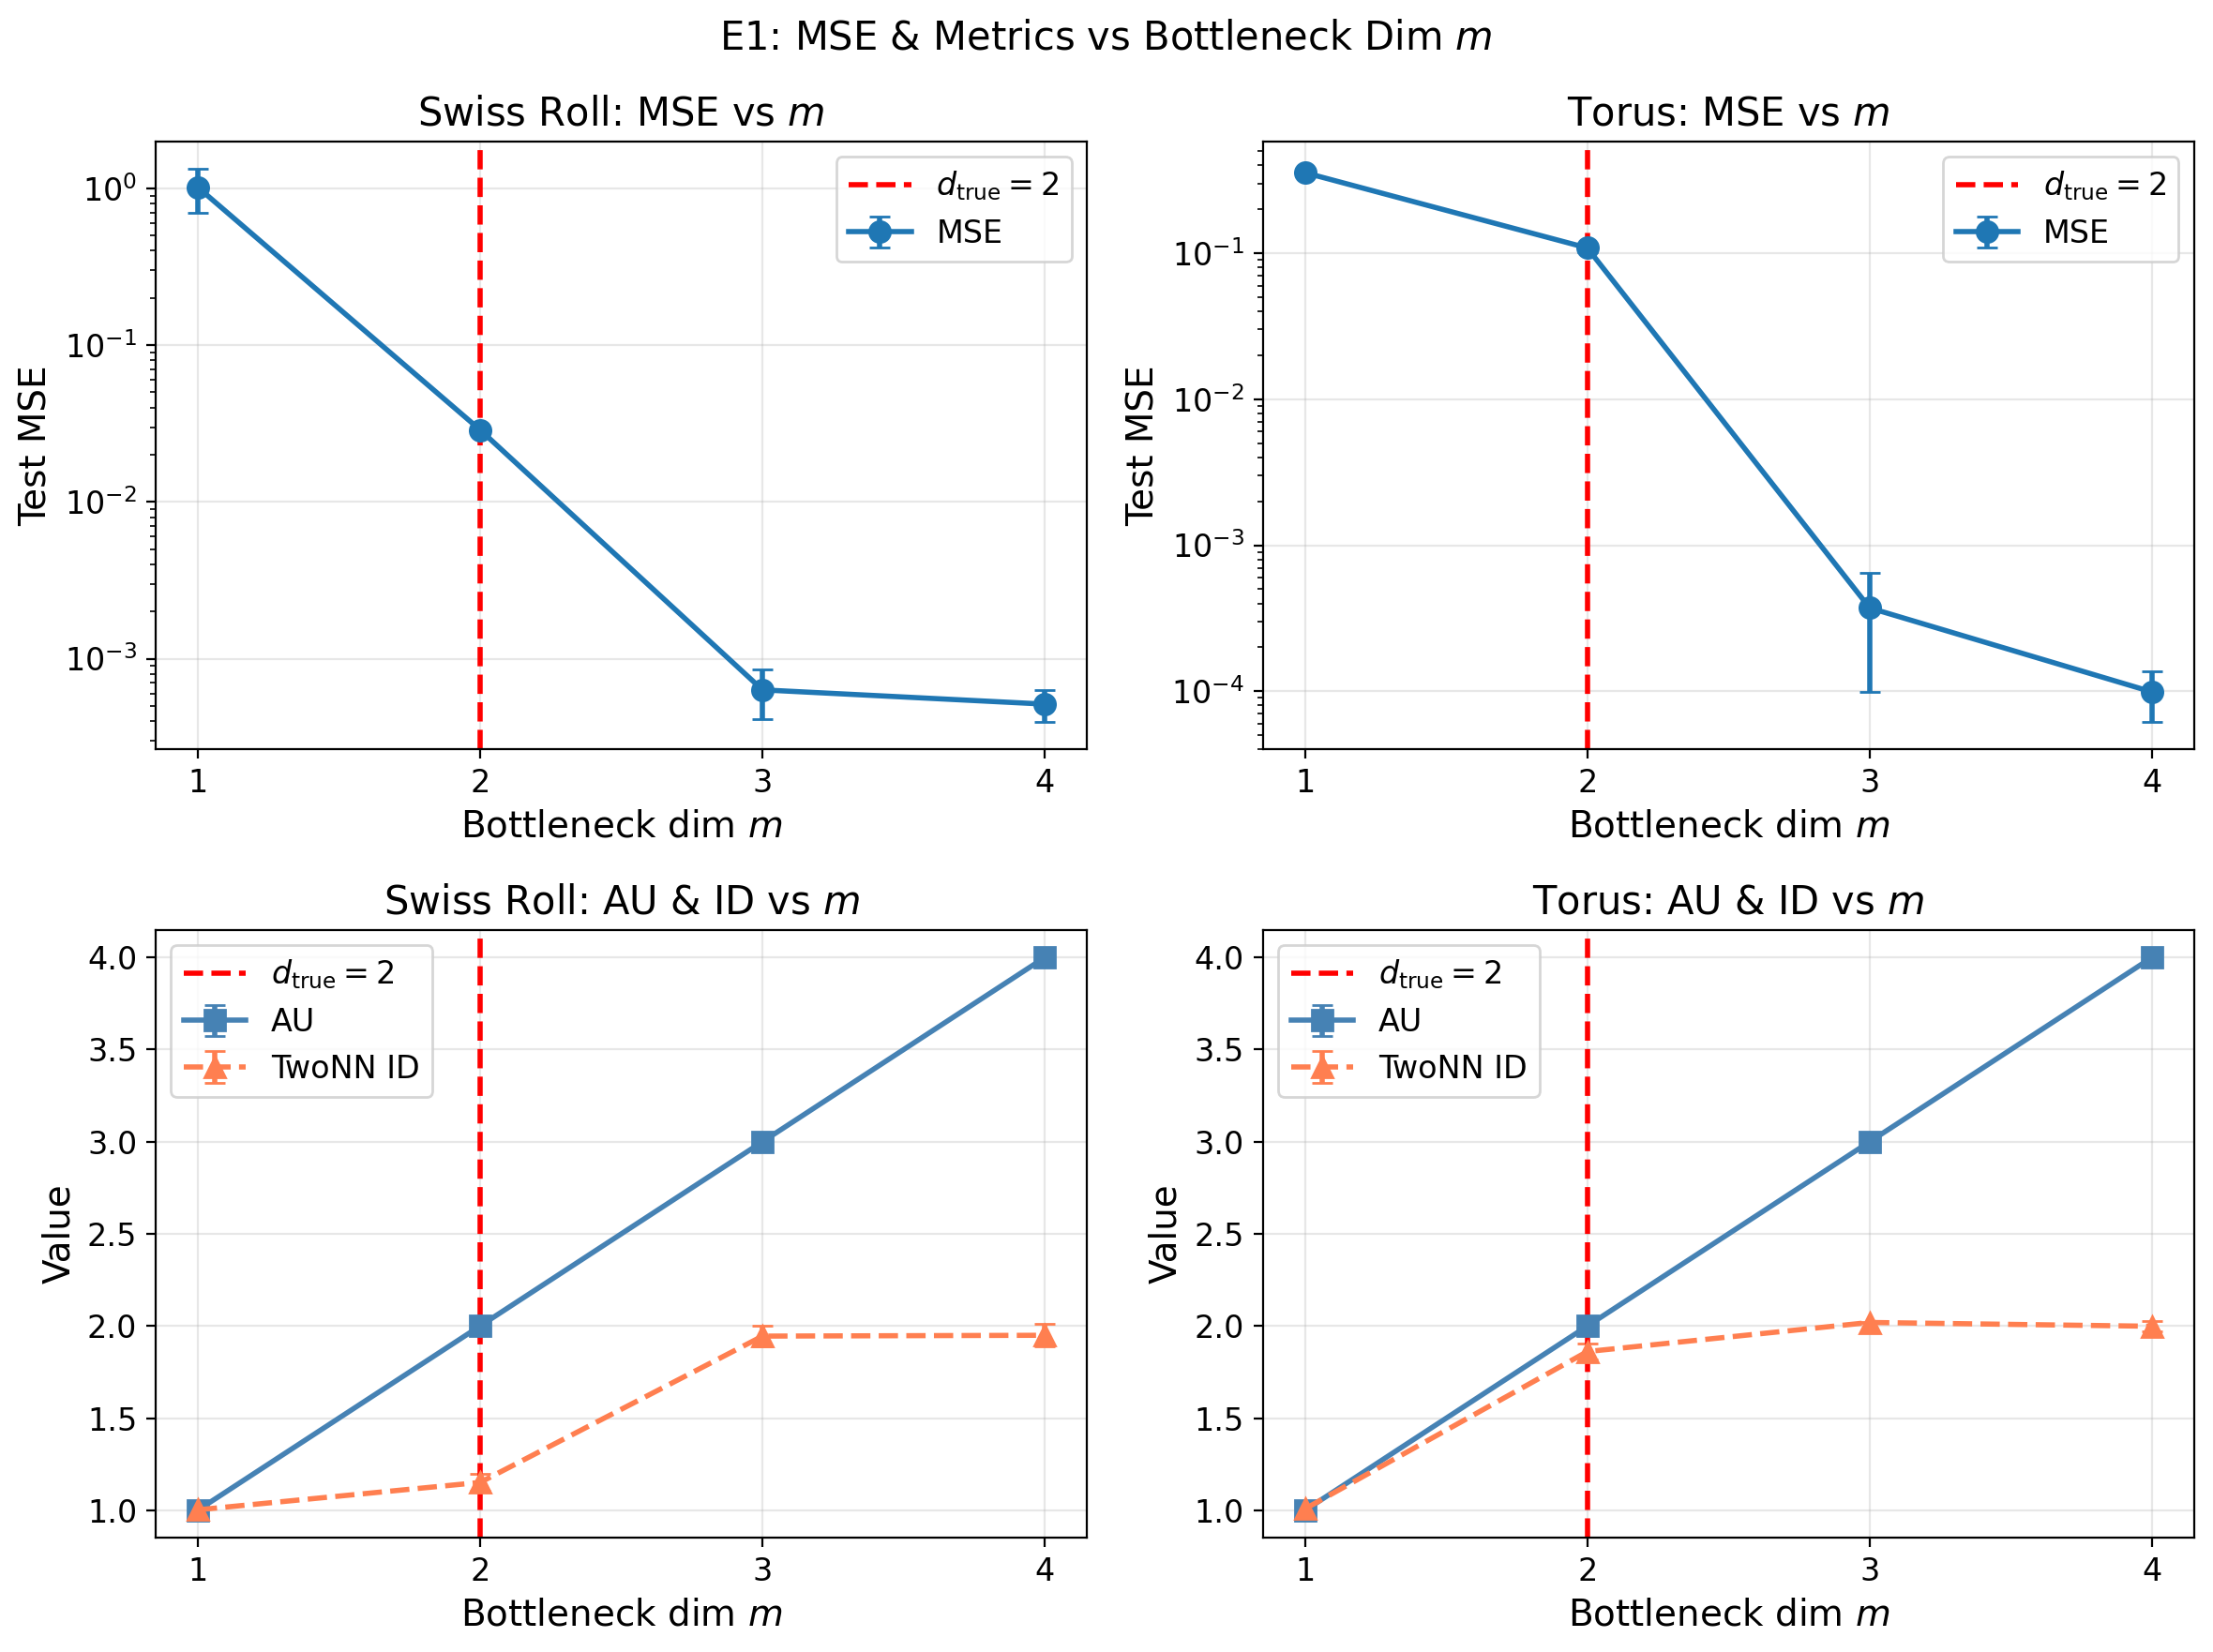
\includegraphics[width=0.92\linewidth]{../results/figures/E1_mse_vs_m.png}
\caption{E1: MSE vs.\ $m$ (3-seed mean$\pm$std, log scale). Swiss Roll (solid, $\bullet$): sharp drop at $m=2=\dtrue$. Torus (dashed, $\blacktriangle$): effective elbow at $m=3$.}
\label{fig:e1_mse}
\end{figure}

\subsubsection{Decoder Jacobian Analysis (Experiment E2)}

Decoder Jacobian singular value spectra were evaluated (significant singular value count, condition number $\kap$, and TSA error) as shown in Table~\ref{tab:e2}.

\begin{table}[!t]
\centering
\caption{E2: Decoder Jacobian Analysis}
\label{tab:e2}
\begin{tabular}{lrccc}
\toprule
Manifold & $m$ & Sig.\ SVs & $\kap$ & TSA error ($^\circ$) \\
\midrule
\multirow{4}{*}{Swiss Roll} & 1 & 1.00 & 1.00 & 26.2 \\
 & \textbf{2} & \textbf{2.00} & 1.51 & 44.3 \\
 & 3 & 3.00 & 1.75 & 38.9 \\
 & 4 & 3.00 & 2.03 & 43.6 \\
\midrule
\multirow{4}{*}{Torus} & 1 & 1.00 & 1.00 & 10.6 \\
 & \textbf{2} & \textbf{2.00} & 2.30 & 21.8 \\
 & 3 & 3.00 & 1.50 & 22.0 \\
 & 4 & 3.00 & 1.47 & 25.2 \\
\bottomrule
\end{tabular}
\end{table}

For Torus at $m=4$, the significant singular value count is 3.00 (not 4), confirming Proposition~\ref{thm:rank}: the surplus dimension degenerates to match the topological embedding dimension $\demb = 3$.

\subsubsection{Noise Selectivity (Experiment E3)}

We measured the noise selectivity ratio (NSR) $=$ tangent-direction error / normal-direction error for Swiss Roll ($\sigma = 0.1$).
Results are shown in Table~\ref{tab:e3}.

\begin{table}[!t]
\centering
\caption{E3: NSR Analysis (Swiss Roll, $\sigma=0.1$)}
\label{tab:e3}
\begin{tabular}{rcccc}
\toprule
$m$ & NSR mean & NSR median & Tangent err. & Normal err. \\
\midrule
1 & 6.19 & 0.586 & 0.153 & 0.128 \\
\textbf{2} & \textbf{1.01} & \textbf{0.562} & \textbf{0.079} & \textbf{0.126} \\
3 & 1.48 & 1.010 & 0.121 & 0.127 \\
4 & 1.46 & 0.988 & 0.120 & 0.129 \\
\bottomrule
\end{tabular}
\end{table}

At $m=2=\dtrue$, normal-direction error ($0.126$) $>$ tangent-direction error ($0.079$), confirming Proposition~\ref{thm:nsr}.
For $m > \dtrue$, surplus dimensions absorb normal-direction noise and selectivity decreases (NSR $\approx 1.5$).

\subsubsection{Trustworthiness vs.\ Bottleneck Dimension (Experiment E5)}\label{sec:exp_e5}

Table~\ref{tab:e5} and Fig.~\ref{fig:e5} quantify the $m$-dependence of Trustworthiness.

\begin{table}[!t]
\centering
\caption{E5: Trustworthiness vs.\ $m$ (3-seed mean$\pm$std, $k=10$)}
\label{tab:e5}
\begin{tabular}{rcc}
\toprule
$m$ & Swiss Roll ($\dtrue=2$) & Torus ($\dtrue=2$, $\demb=3$) \\
\midrule
1 & $0.9838\pm0.0062$ & $0.9395\pm0.0043$ \\
\textbf{2} & $\boldsymbol{0.9990\pm0.0000}$ $\leftarrow$ & $0.9847\pm0.0018$ \\
\textbf{3} & $0.9995\pm0.0001$ & $\boldsymbol{0.9996\pm0.0001}$ $\leftarrow$ \\
4 & $0.9993\pm0.0001$ & $0.9995\pm0.0002$ \\
\bottomrule
\end{tabular}
\end{table}

Swiss Roll: Trustworthiness jumps from $0.984 \to 0.999$ at $m=1 \to 2$ ($\Delta \approx 0.015$); further increases are $< 0.001$.
Torus: maximum improvement at $m=2 \to 3$ ($\Delta \approx 0.015$), consistent with $\demb = 3$ (Proposition~\ref{thm:trust}).

\begin{figure}[!t]
\centering
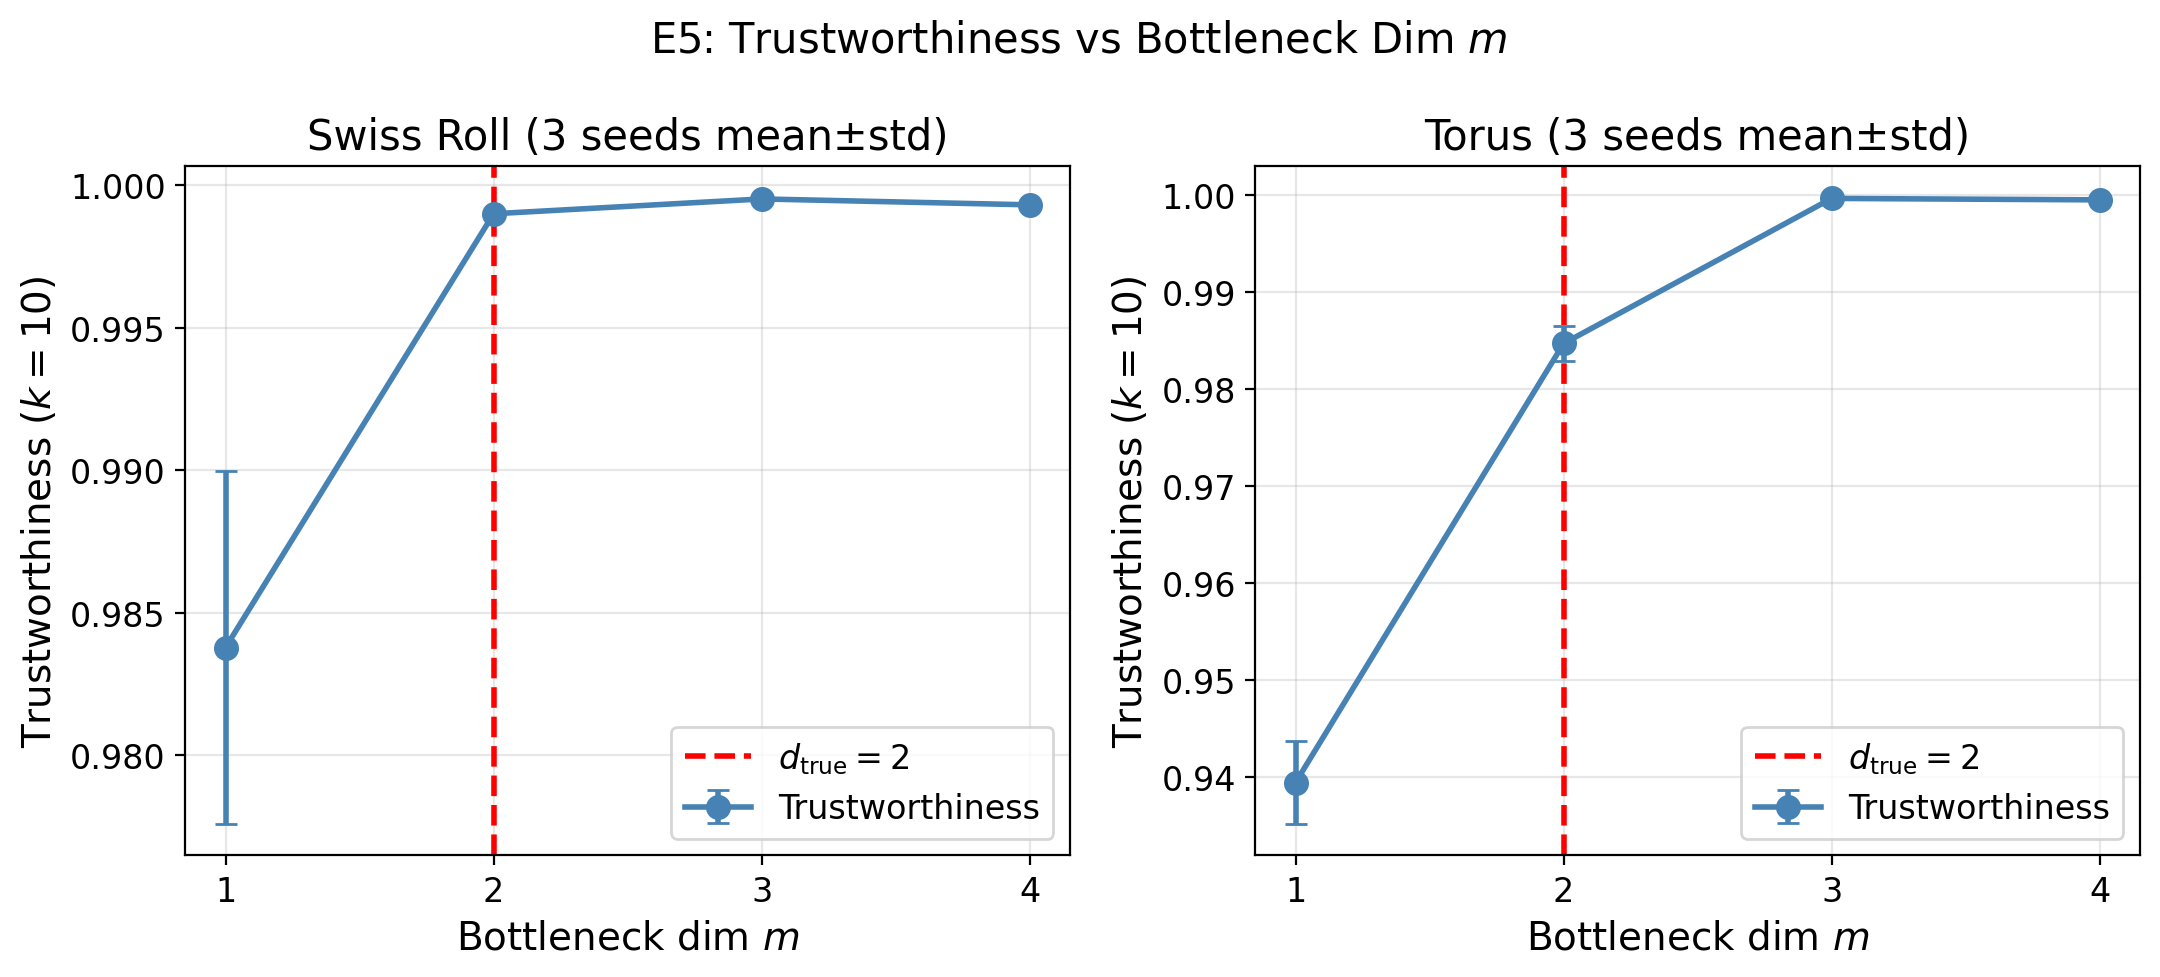
\includegraphics[width=0.92\linewidth]{../results/figures/E5_trustworthiness.png}
\caption{E5: Trustworthiness vs.\ $m$ (3-seed mean$\pm$std). Swiss Roll (left): sharp improvement at $m=2$. Torus (right): sharp improvement at $m=3=\demb$.}
\label{fig:e5}
\end{figure}

\subsection{Information Bottleneck and Topological Embedding (RQ2, RQ3)}\label{sec:exp_topology}

\textbf{Question answered (RQ2, RQ3):} Does KL-regularized AU saturation reflect the topological minimum embedding dimension? Is decoder isometry ($\kap \approx 1$) achievable?

\subsubsection{AU Saturation via Information Bottleneck (Experiment EA)}

Tables~\ref{tab:ea} and~\ref{tab:ea_torus} compare AU($m$) for Vanilla AE, AE+L2, and VAE ($\beta=4$) on Swiss Roll and Torus.

\begin{table}[!t]
\centering
\caption{EA: Swiss Roll VAE AU vs.\ $m$ (3-seed mean$\pm$std, $\beta=4$)}
\label{tab:ea}
\begin{tabular}{rcc}
\toprule
$m$ & VAE (AU) & VAE MSE \\
\midrule
1  & $1.0\pm0.0$ & $1.492\pm0.257$ \\
2  & $2.0\pm0.0$ & $0.070\pm0.012$ \\
3  & $\boldsymbol{2.0\pm0.0}$ $\leftarrow$ sat. & $0.054\pm0.004$ \\
6  & $\boldsymbol{2.0\pm0.0}$ & $0.043\pm0.006$ \\
12 & $\boldsymbol{2.0\pm0.0}$ & $0.040\pm0.003$ \\
16 & $\boldsymbol{2.0\pm0.0}$ & $0.037\pm0.003$ \\
\bottomrule
\end{tabular}
\end{table}

\begin{table}[!t]
\centering
\caption{EA: Torus VAE AU vs.\ $m$ (3-seed mean$\pm$std, $\beta=4$)}
\label{tab:ea_torus}
\begin{tabular}{rcc}
\toprule
$m$ & VAE (AU) & VAE MSE \\
\midrule
1  & $1.0\pm0.0$ & $0.565\pm0.029$ \\
2  & $2.0\pm0.0$ & $0.299\pm0.009$ \\
4  & $2.0\pm0.0$ & $0.219\pm0.005$ \\
6  & $\boldsymbol{3.0\pm0.0}$ $\leftarrow$ sat. & $0.074\pm0.010$ \\
12 & $\boldsymbol{3.0\pm0.0}$ & $0.016\pm0.001$ \\
16 & $\boldsymbol{3.0\pm0.0}$ & $0.010\pm0.001$ \\
\bottomrule
\end{tabular}
\end{table}

For Swiss Roll, VAE AU maintains AU$=2$ (= $\dtrue$) for all $m \geq 2$ with zero standard deviation across all 3 seeds---a strong evidence of robustness.
For Torus, VAE AU saturates at $3 > \dtrue = 2$ for $m \geq 6$, corresponding to the topological minimum embedding dimension of 3.
Vanilla AE always has AU$=m$ (confirmed in single-seed experiments), confirming Proposition~\ref{thm:au}: AU saturation requires KL regularization.

\begin{figure}[!t]
\centering
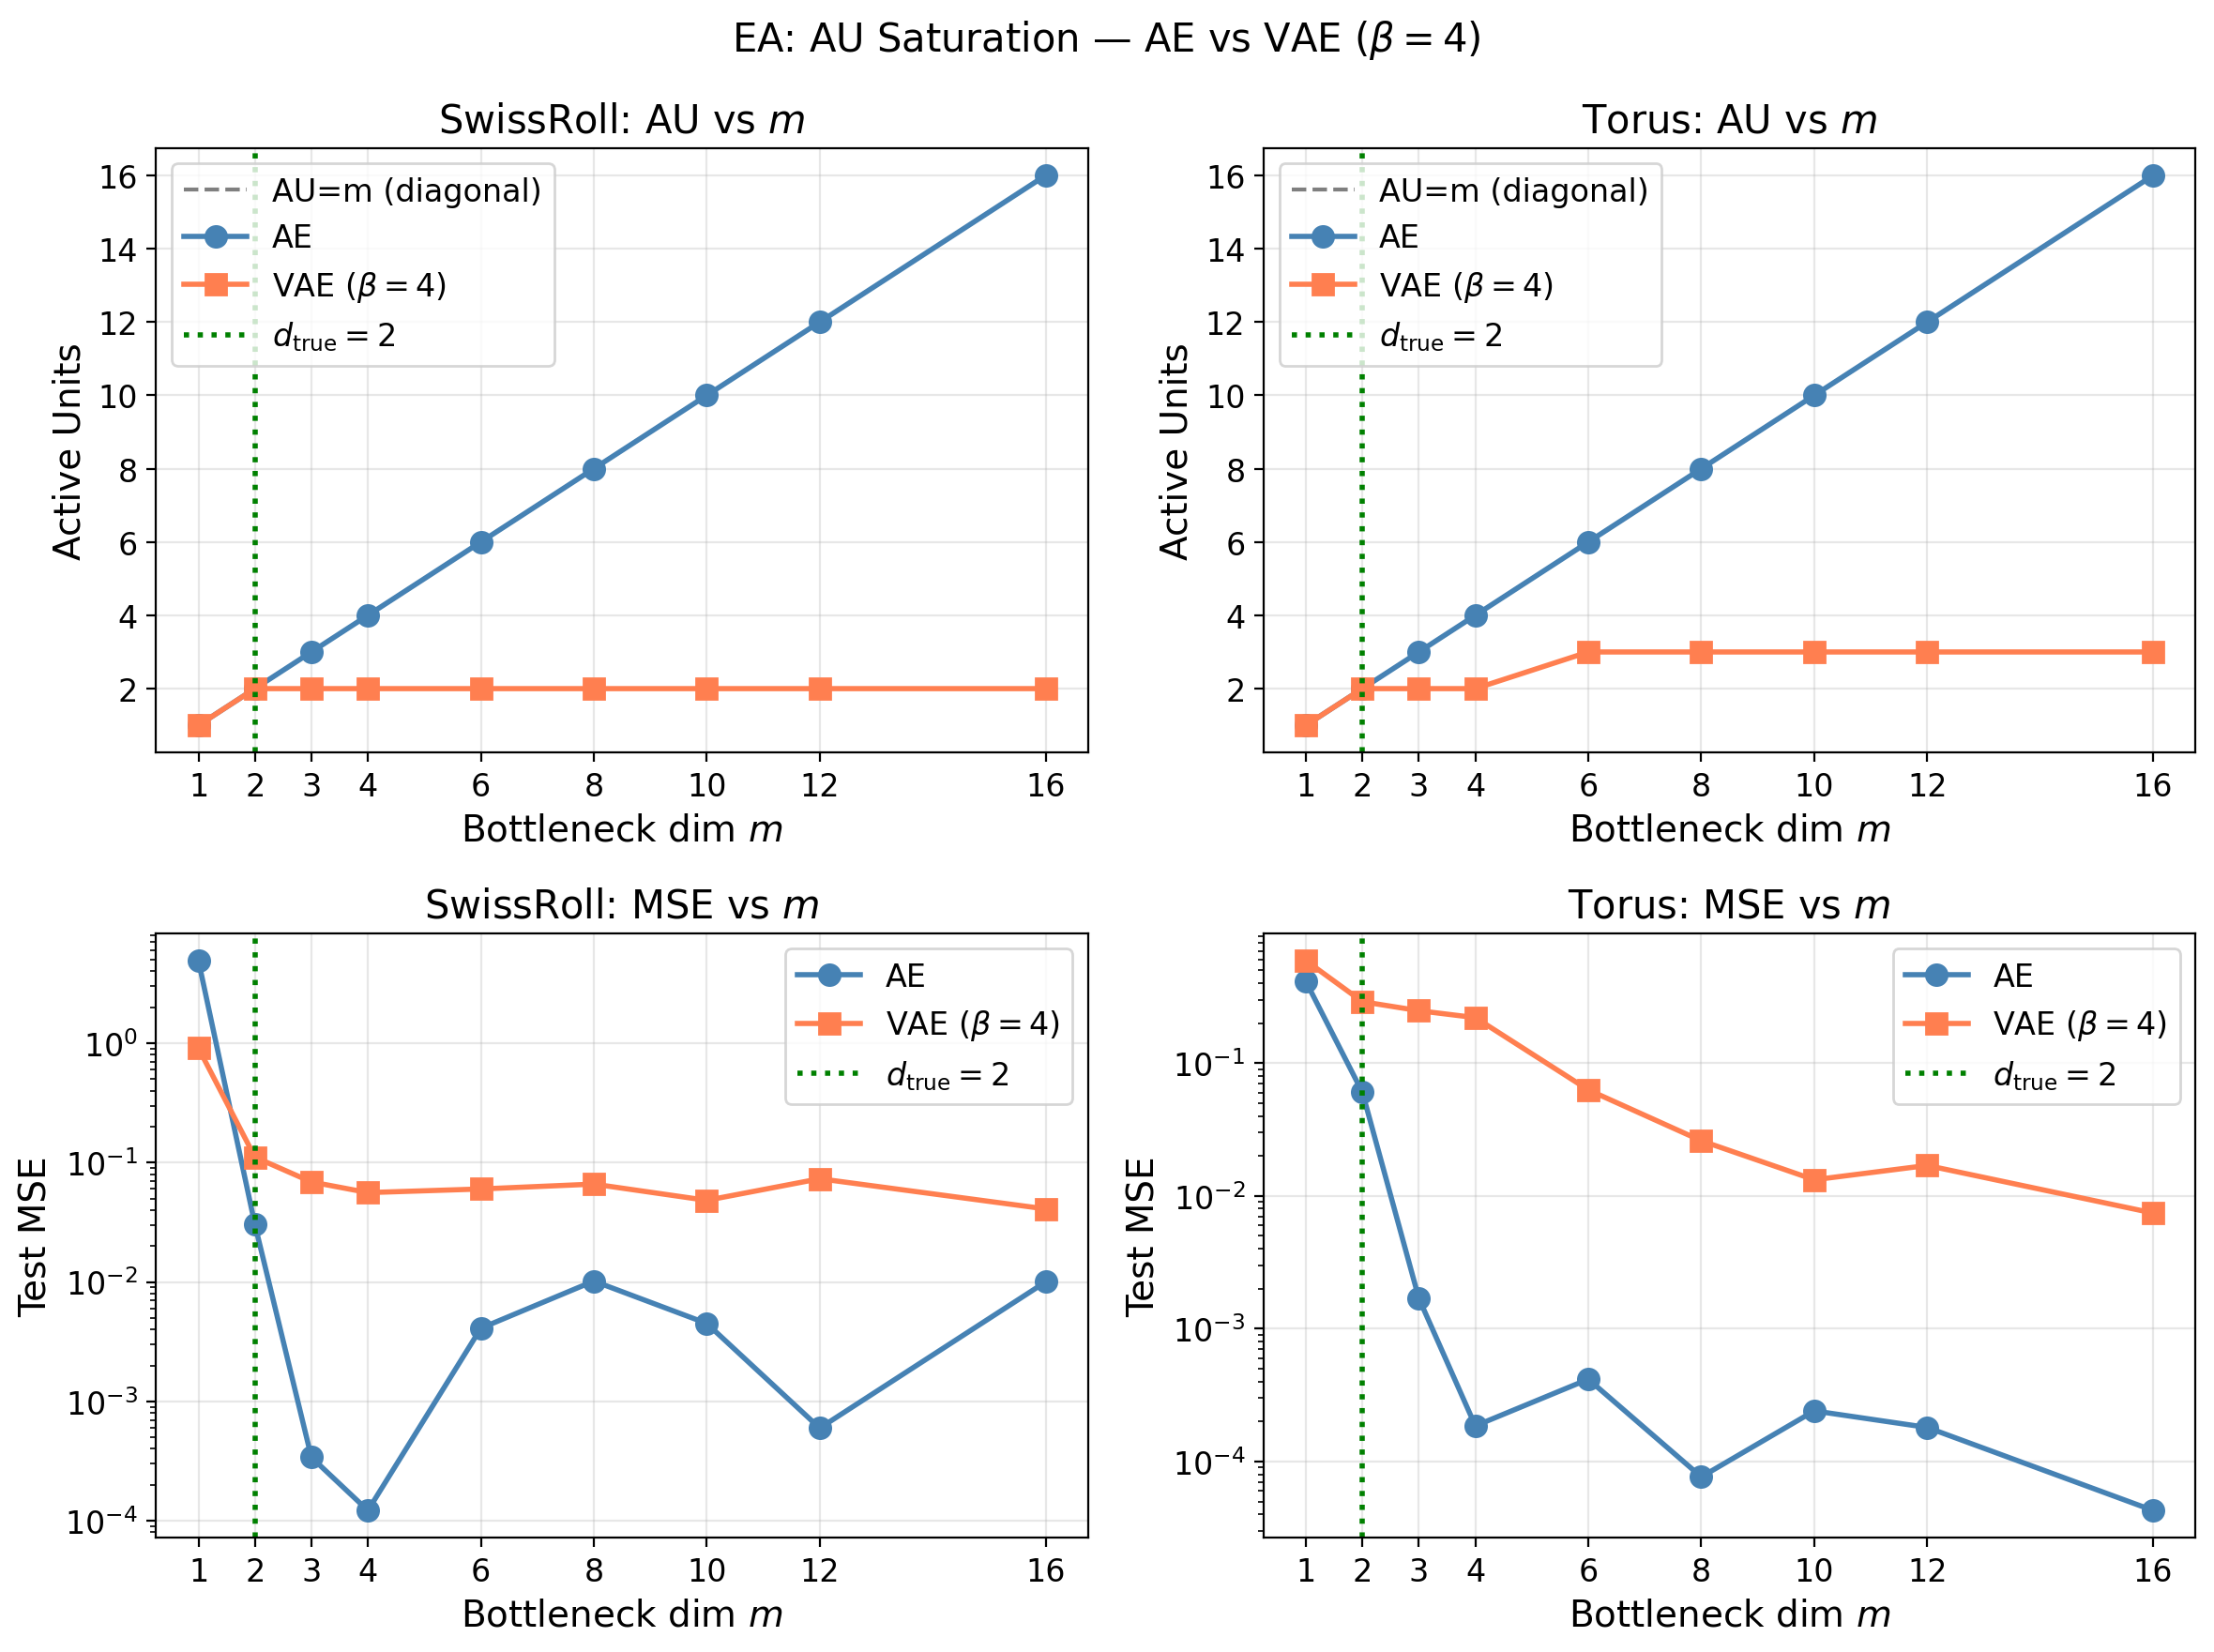
\includegraphics[width=0.92\linewidth]{../results/figures/EA_au_saturation.png}
\caption{EA: AU vs.\ $m$ for Swiss Roll (AE vs.\ VAE). Only VAE exhibits AU saturation at $\dtrue=2$.}
\label{fig:ea}
\end{figure}

\subsubsection{Topological Constraints and AU Saturation (Experiment EB)}\label{sec:exp_eb}

Table~\ref{tab:eb} compares $\AUsat$ with the topological minimum embedding dimension for four synthetic manifolds.

\begin{table}[!t]
\centering
\caption{EB: Topological AU Experiment (VAE $\beta=4$, standardized inputs). \checkmark: $\AUsat =$ topological embedding dim. (main result). $\times$: exception (preprocessing-dependent). $\triangle$: conditional.}
\label{tab:eb}
\begin{tabular}{lcccc}
\toprule
Manifold & $\dtrue$ & $\pi_1$ & Topol.\ $\demb$ & VAE $\AUsat$ \\
\midrule
Torus $T^2$  & 2 & $\mathbb{Z}^2$ & 3 & 3 \checkmark \\
M\"{o}bius Band & 2 & $\mathbb{Z}$ & 3 & 3 \checkmark \\
Swiss Roll   & 2 & $\{1\}$ & 2 & 3 $\times$ \\
Circle $S^1$ & 1 & $\mathbb{Z}$ & 2 & 2 ($m\geq6$) $\triangle$ \\
\bottomrule
\end{tabular}
\end{table}

Torus and M\"{o}bius Band show $\AUsat = \demb = 3$ (\checkmark: main result).
Swiss Roll shows $\AUsat = 3 \neq \demb = 2$ under standardization ($\times$: preprocessing-dependent exception; in Exp.\ EA without standardization $\AUsat = 2$ was observed).
Circle $S^1$ requires $m \geq 6$ to observe $\AUsat = 2$ ($\triangle$: grid-resolution limited).

\textbf{Note on preprocessing dependence:}
Experiment EB uses component-wise standardization (mean 0, variance 1), while EA uses the original scale.
The Swiss Roll $\AUsat$ changing from 2 (EA) to 3 (EB under standardization) shows that $\AUsat$ is sensitive to input scale---it is not a preprocessing-invariant topological invariant.
The main result (Torus, M\"{o}bius Band) should be reproduced under the same standardization protocol.

\begin{figure}[!t]
\centering
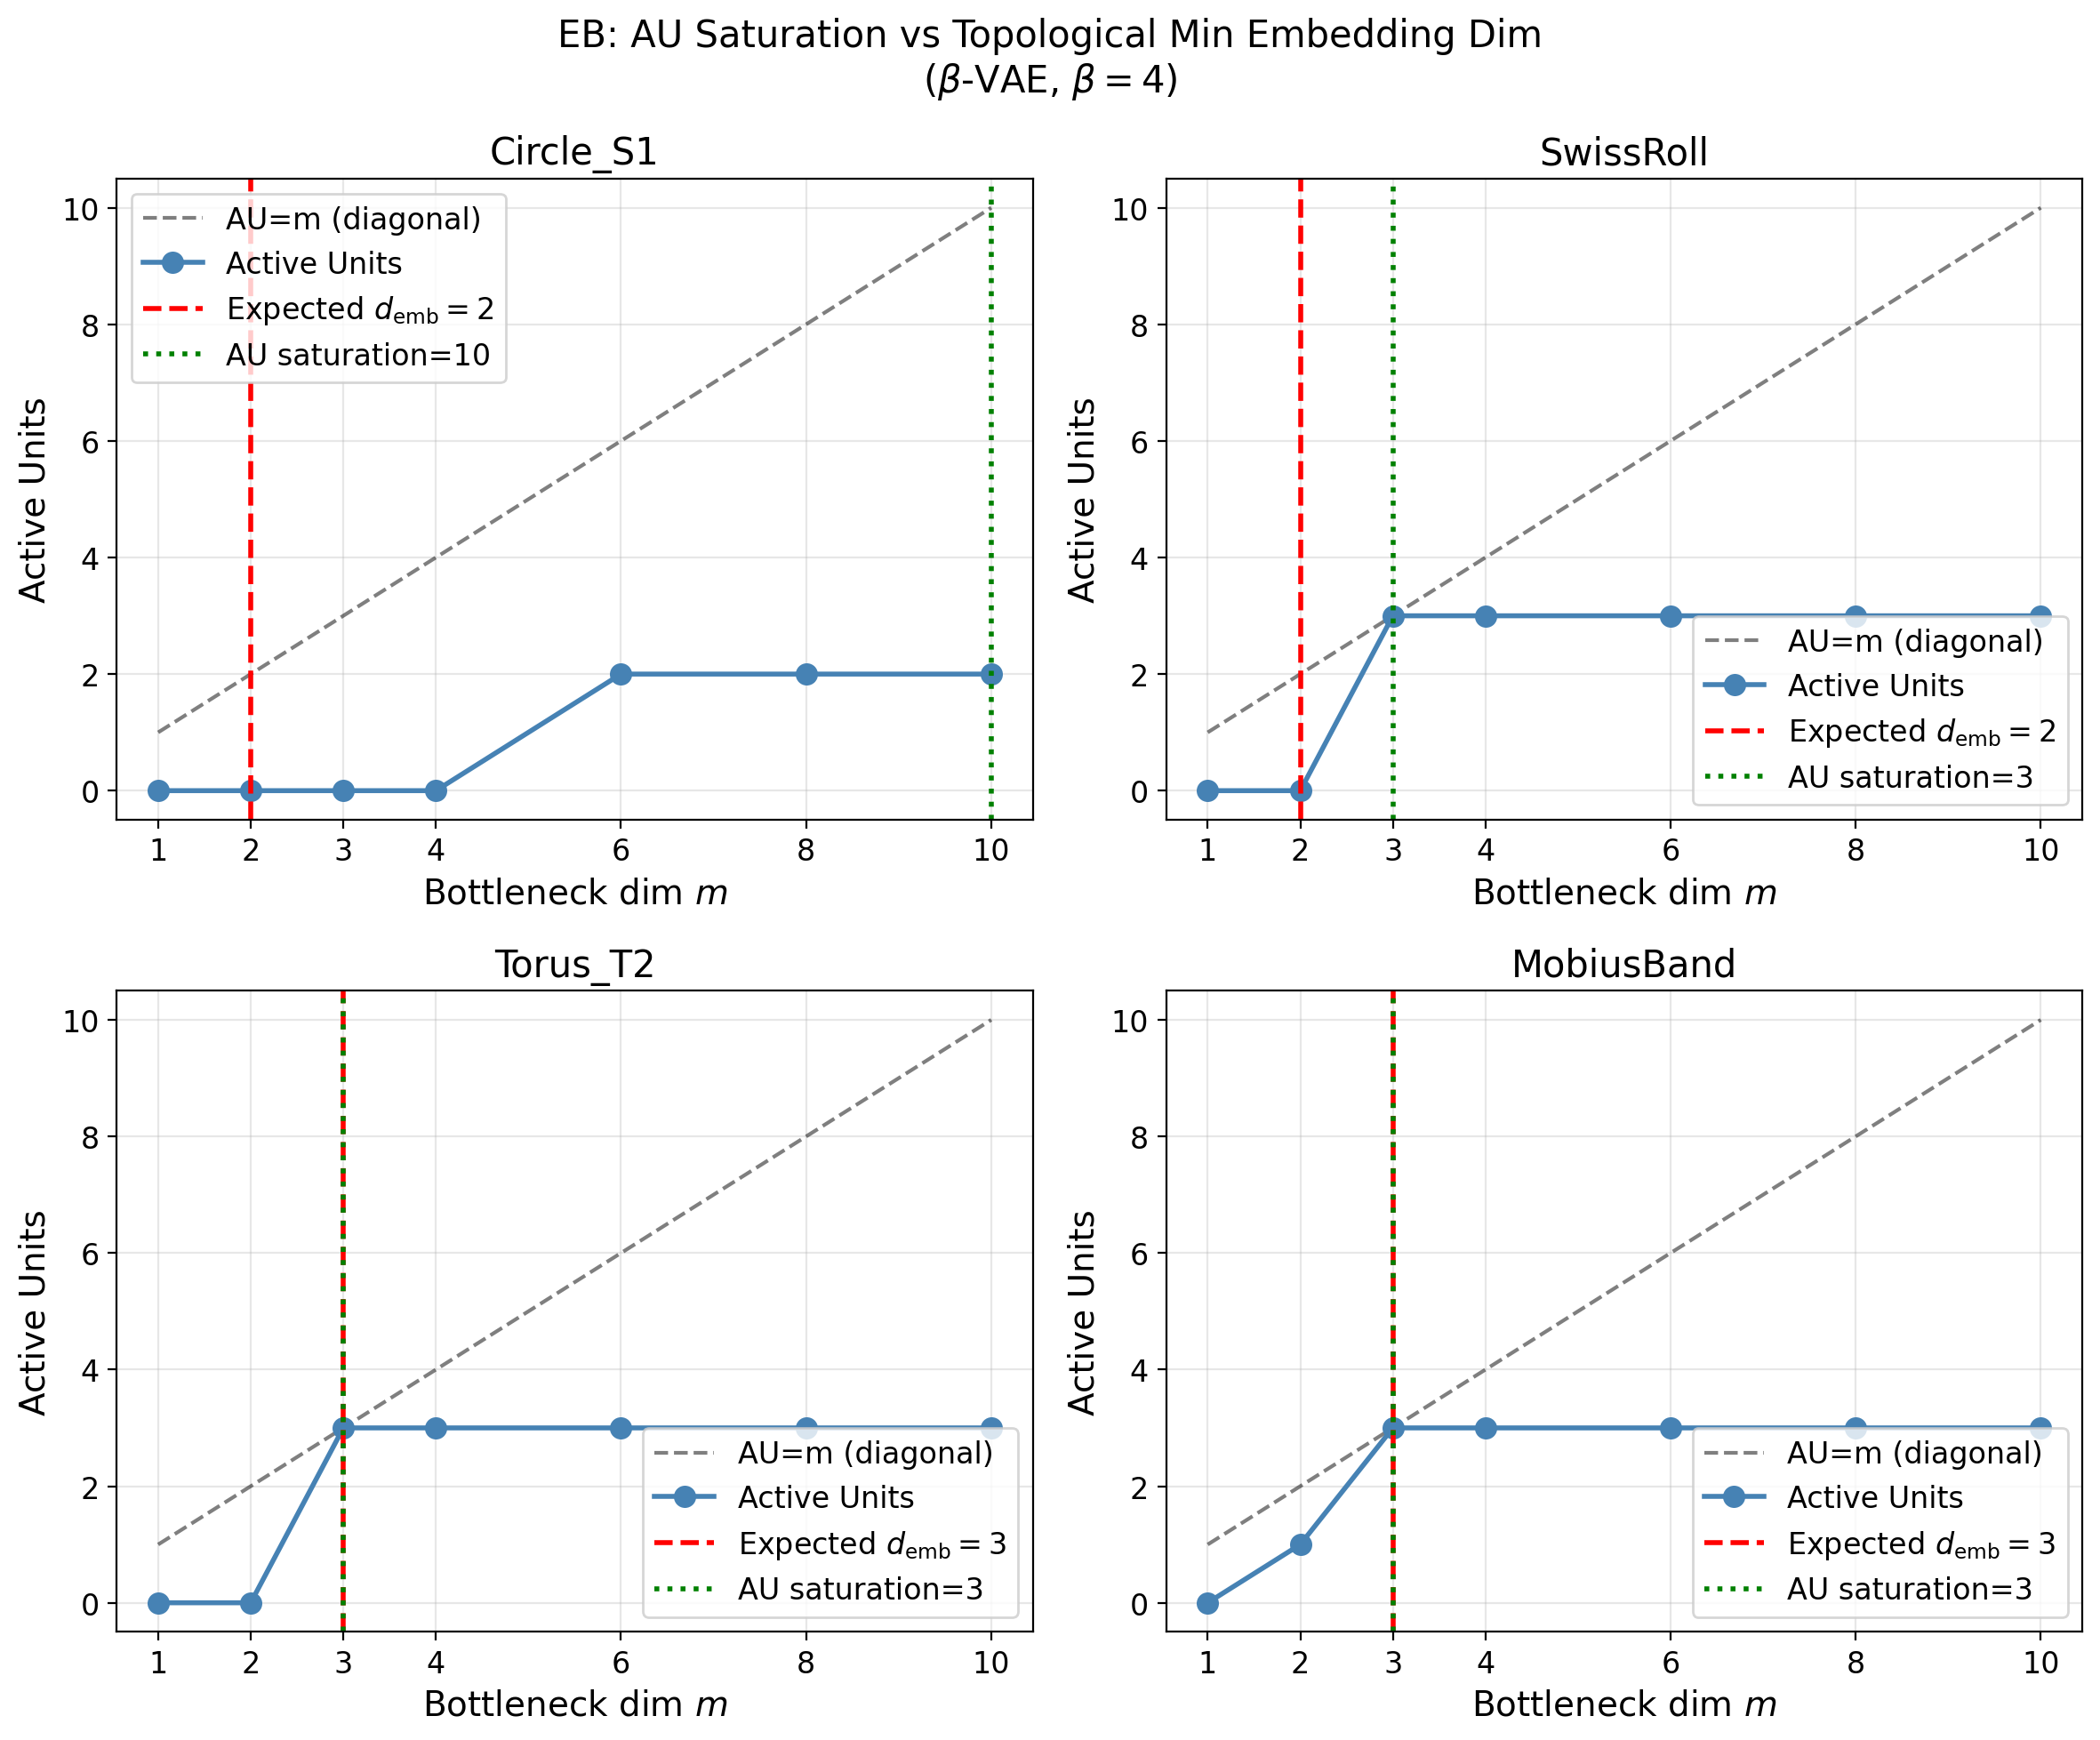
\includegraphics[width=0.92\linewidth]{../results/figures/EB_topology_au.png}
\caption{EB: VAE AU saturation for four manifolds (standardized inputs). Torus and M\"{o}bius Band (\checkmark) are the main results. Swiss Roll ($\times$) and Circle $S^1$ ($\triangle$) are conditional exceptions.}
\label{fig:eb}
\end{figure}

\subsubsection{Isometric Embedding via Decoder Regularization (Experiment EC)}\label{sec:exp_ec}

\textbf{Isometry is a prerequisite for reliable ID estimation in latent space:}
TwoNN/MLE estimates in latent space are reliable only when the decoder $g: \R^m \to \R^N$ preserves the distance structure of the data manifold without distortion (isometric embedding), i.e., when $\kap \approx 1$ (Theorem~\ref{thm:pullback}).

The IsometricAE loss function is
\begin{equation}
  \mathcal{L}_\mathrm{iso} = \mathcal{L}_\mathrm{rec}
  + \lambda_\mathrm{iso} \cdot \frac{1}{n}\sum_{i=1}^{n}
    \|\Jg(z_i)^\top \Jg(z_i) - I_m\|_F^2
  \label{eq:iso_loss}
\end{equation}
with $\lambda_\mathrm{iso} = 0.01$.

Table~\ref{tab:ec} compares four models on Swiss Roll ($m=2$, 200 epochs).

\begin{table}[!t]
\centering
\caption{EC: IsometricAE Comparison (Swiss Roll, $m=2$, 3-seed mean$\pm$std)}
\label{tab:ec}
\begin{tabular}{lccc}
\toprule
Model & MSE & $\kap$ & Trust. \\
\midrule
AE          & $0.028\pm0.001$ & $1.433\pm0.182$ & $0.999\pm0.000$ \\
CAE         & $0.029\pm0.001$ & $1.907\pm0.059$ & $0.999\pm0.000$ \\
\textbf{IsometricAE} & $0.028\pm0.001$ & $\boldsymbol{1.055\pm0.005}$ & $0.999\pm0.000$ \\
DAE         & $0.030\pm0.002$ & $1.431\pm0.144$ & $0.999\pm0.000$ \\
\bottomrule
\end{tabular}
\end{table}

IsometricAE achieves the lowest condition number $\kap = 1.055\pm0.005$, confirming Theorem~\ref{thm:pullback}.
The standard deviation of $0.005$ indicates high reproducibility across seeds.
CAE shows the highest $\kap = 1.907\pm0.059$---encoder-side Jacobian regularization unexpectedly distorts the decoder pullback metric.
All models achieve Trustworthiness $= 0.9990\pm0.0000$, showing that neighborhood preservation is equivalent across model types at the correct $m$.

\begin{figure}[!t]
\centering
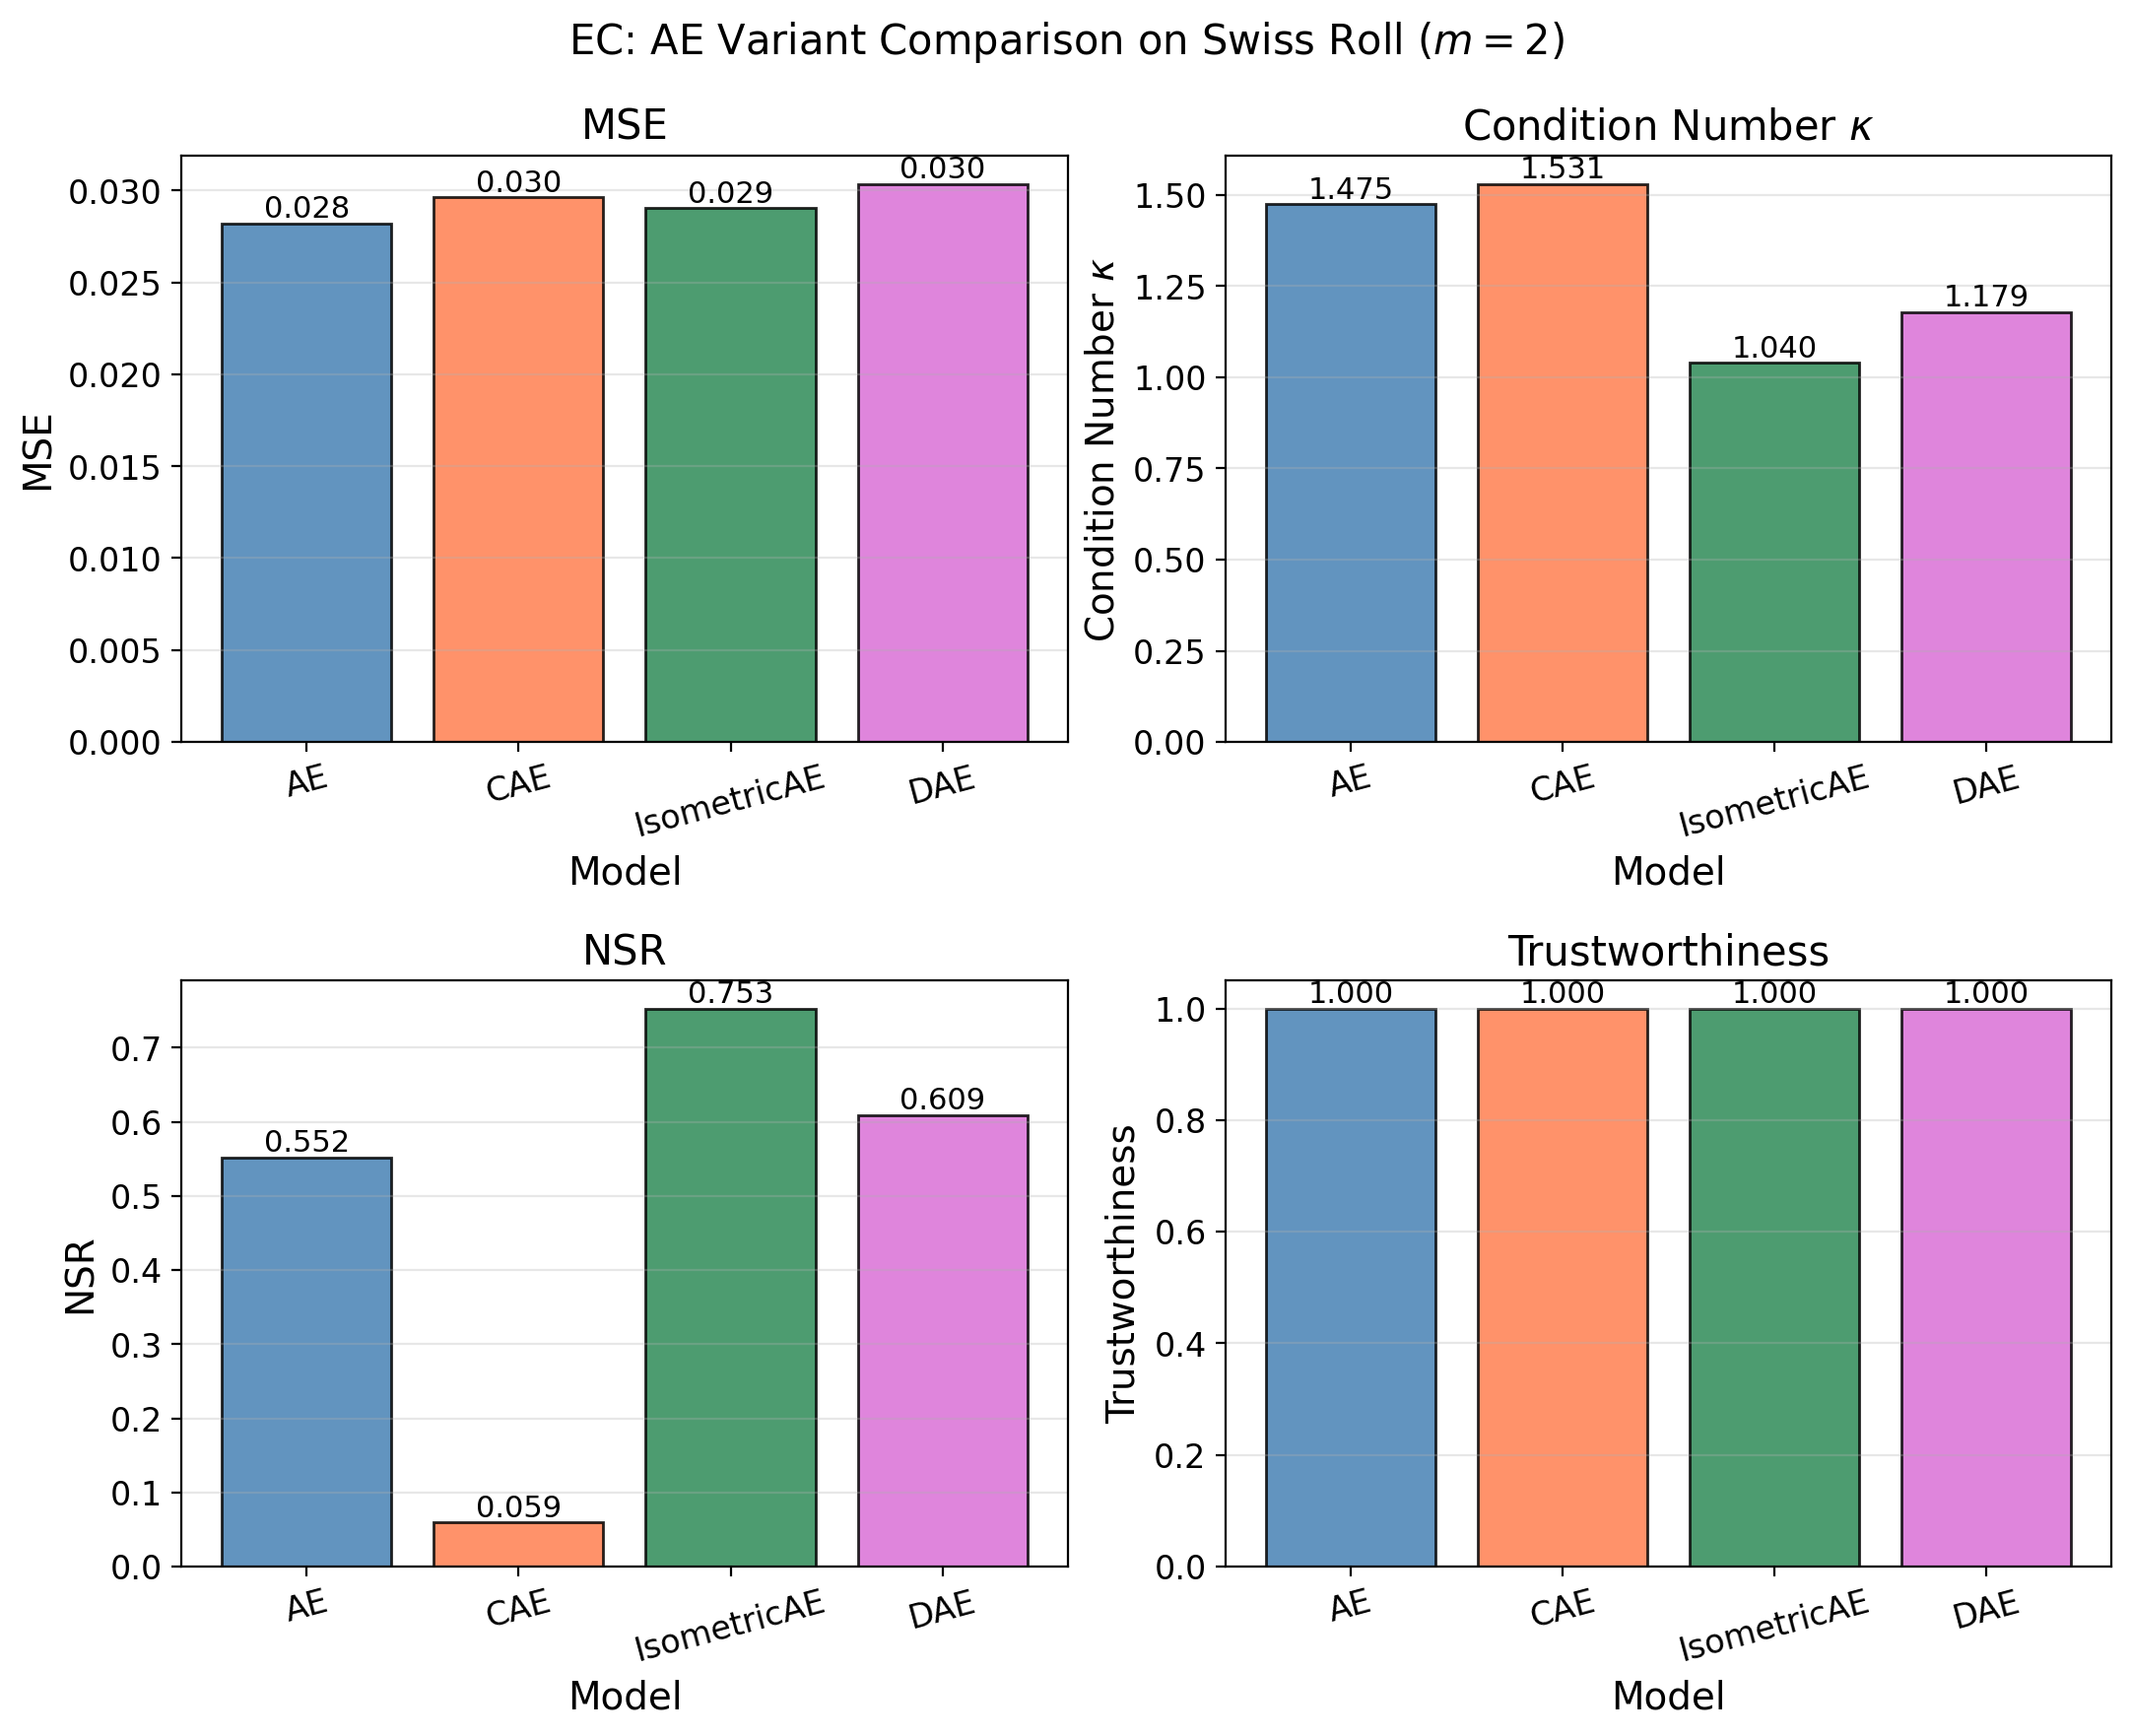
\includegraphics[width=0.92\linewidth]{../results/figures/EC_isometric_comparison.png}
\caption{EC: Condition number $\kap$ comparison. IsometricAE achieves the lowest $\kap \approx 1$.}
\label{fig:ec}
\end{figure}

\subsection{Application to MNIST (RQ1 + Novel Finding)}\label{sec:exp_mnist}

\textbf{Question (RQ1 on real data + secondary finding):} Does the ID estimation framework provide useful design guidance for real image data (MNIST)? What learning dynamics emerge (E6)?

MNIST (10 handwritten digit classes) has a complex manifold structure: each class forms a separate sub-manifold, creating what we term \emph{Manifold Entanglement}~\cite{carlsson2009topology}---the support $\mathcal{X} = \bigcup_{k=0}^{9}\mathcal{M}_k$ cannot be described by a single fundamental group $\pi_1$.
This predicts: (1)~TwoNN underestimation bias amplification, (2)~$\AUsat > \dID$ due to class boundary representation, (3)~smooth MSE decrease (smooth elbow problem).

\subsubsection{MNIST Bottleneck Sweep (Experiment E4)}

We trained AE and VAE ($\beta=4$) on MNIST (train: 20{,}000 samples, test: 3{,}000 samples, 300 epochs) sweeping $m$ from 1 to 256.
Results are shown in Tables~\ref{tab:e4_ae} and~\ref{tab:e4_vae}.

\begin{table}[!t]
\centering
\caption{E4: MNIST AE Results (300 epochs). TwoNN ID and MLE ID converge for $m \geq 64$, indicating effective ID $\approx 10$--12.}
\label{tab:e4_ae}
\begin{tabular}{rccccc}
\toprule
$m$ & MSE & AU & TwoNN ID & MLE ID & CKA \\
\midrule
1   & 0.0437 & 1   & 1.02  & 1.15  & 0.102 \\
4   & 0.0292 & 4   & 3.86  & 4.29  & 0.575 \\
8   & 0.0191 & 8   & 6.08  & 6.70  & 0.725 \\
12  & 0.0148 & 12  & 7.59  & 7.94  & 0.791 \\
16  & 0.0121 & 16  & 7.96  & 8.61  & 0.812 \\
32  & 0.0087 & 32  & 8.84  & 9.89  & 0.875 \\
64  & 0.0062 & 64  & 9.54  & 11.26 & 0.908 \\
128 & 0.0061 & 128 & 9.84  & 11.45 & 0.921 \\
256 & 0.0057 & 256 & 10.02 & 11.85 & 0.953 \\
\bottomrule
\end{tabular}
\end{table}

\begin{table}[!t]
\centering
\caption{E4: MNIST VAE ($\beta=4$) Results (300 epochs). At $m=12$, AU growth rate drops sharply ($m^\mathrm{knee}=12$, AU$=8$). MNIST is gradual-type, so $m^\mathrm{knee} \neq \AUsat$.}
\label{tab:e4_vae}
\begin{tabular}{rcccc}
\toprule
$m$ & MSE & AU & TwoNN ID & MLE ID \\
\midrule
1   & 0.0464 & 1  & 1.00 & 1.11 \\
4   & 0.0275 & 4  & 3.72 & 4.28 \\
8   & 0.0186 & 8  & 6.36 & 6.98 \\
12  & 0.0184 & 8  & 6.26 & 6.97 \\
16  & 0.0148 & 11 & 7.18 & 8.23 \\
32  & 0.0121 & 15 & 8.25 & 9.17 \\
64  & 0.0103 & 29 & 9.16 & 9.87 \\
128 & 0.0085 & 26 & 10.02 & 10.72 \\
256 & 0.0072 & 36 & 10.14 & 11.60 \\
\bottomrule
\end{tabular}
\end{table}

From Table~\ref{tab:e4_ae}, TwoNN ID ($10.02$) and MLE ID ($11.85$) converge near $m \geq 64$, suggesting the effective ID of MNIST is in the range of \textbf{approximately 10--12}.
From Table~\ref{tab:e4_vae}, at $m=12$ the AU growth rate drops sharply ($r(12) = 0/4 = 0.0 < 0.25 \cdot r_\mathrm{max}$), identifying $m^\mathrm{knee} = 12$.
Following the gradual-type design rule (Eq.~\eqref{eq:dzopt_cka_knee}), the practical bottleneck range is $m^* \approx 12$--16, consistent with $\hat{\dID} \approx 10$--12.

The high $\AUsat = 36$ at $m=256$ has multiple possible interpretations: (1) topological complexity from Manifold Entanglement (class boundary representation), or (2) ``capacity leak'' (non-essential style variation absorbed at large $m$).
Distinguishing these requires latent traversal studies or persistent homology analysis, which we leave for future work.

\begin{figure}[!t]
\centering
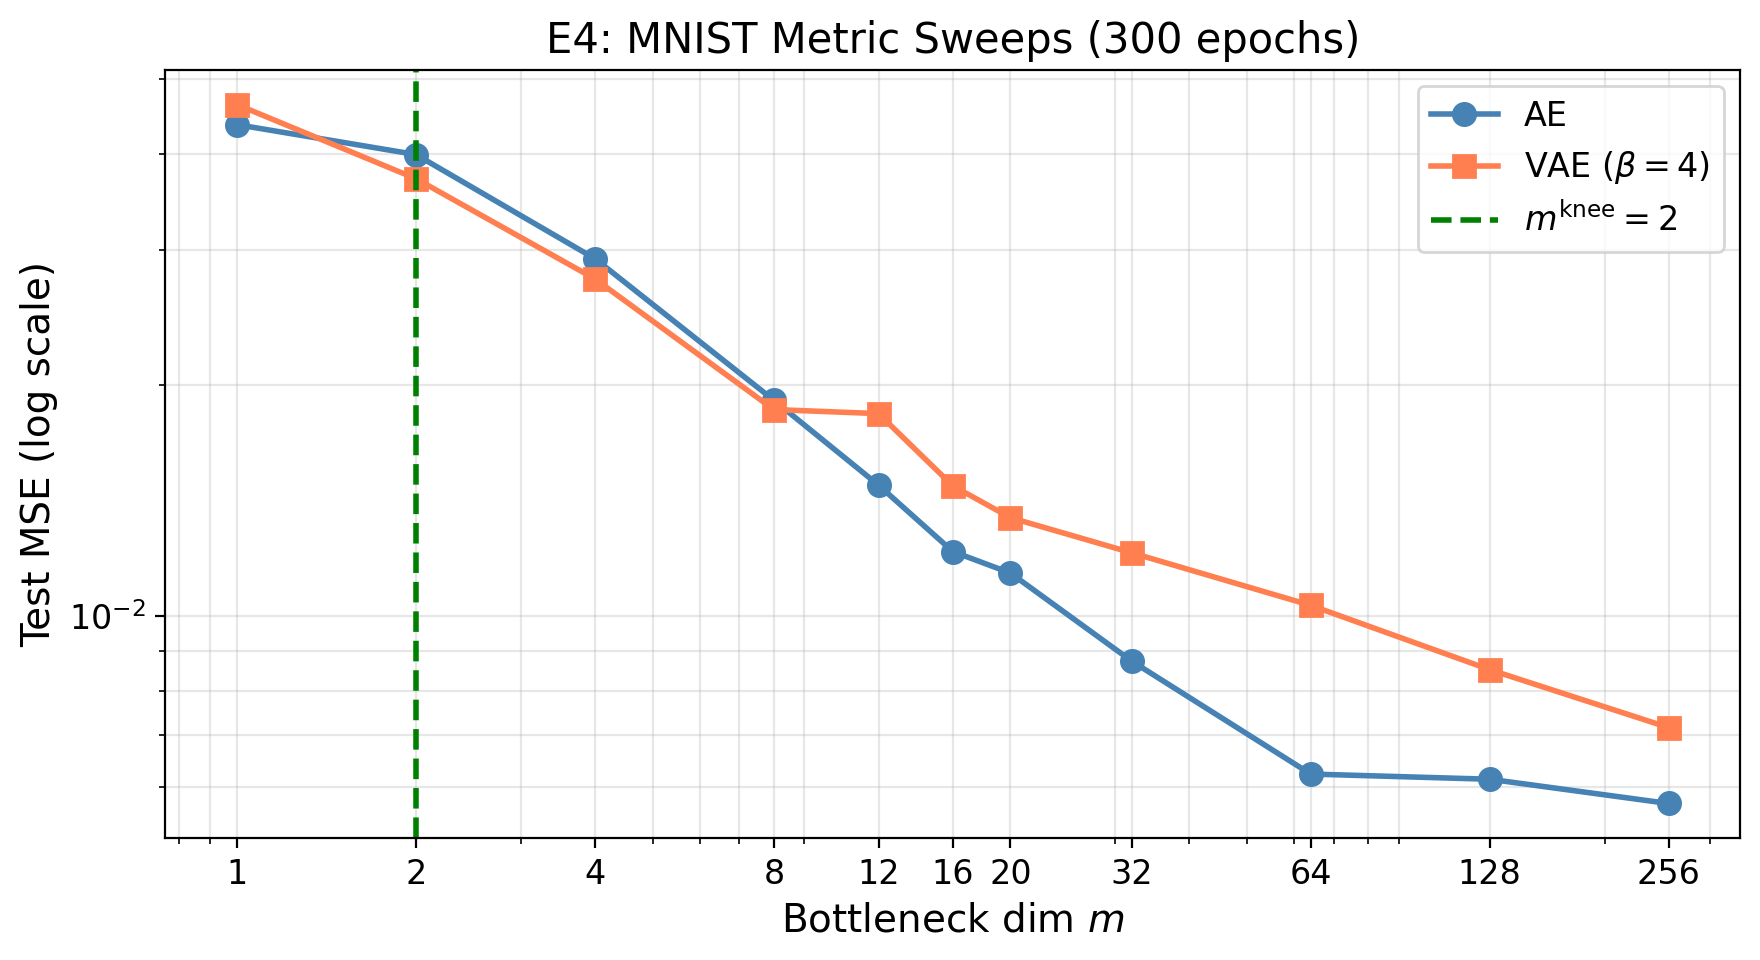
\includegraphics[width=0.92\linewidth]{../results/figures/E4_extended_mse.png}
\caption{E4: MNIST metric sweeps (300 epochs, 20{,}000 training samples). Arrow marks $m^\mathrm{knee}=12$ where VAE AU growth rate drops sharply. MSE shows smooth (no clear elbow) decrease---the smooth elbow problem.}
\label{fig:e4}
\end{figure}

\subsubsection{MNIST Training Dynamics (Experiment E6)}

Table~\ref{tab:e6} tracks Trustworthiness, CKA, and TwoNN ID over 200 epochs for MNIST ($m=16$).

\begin{table}[!t]
\centering
\caption{E6: MNIST Training Dynamics ($m=16$)}
\label{tab:e6}
\begin{tabular}{rcccc}
\toprule
Epoch & MSE (test) & Trustworthiness & CKA & TwoNN ID \\
\midrule
1   & 0.0463 & 0.9263 & 0.785 & 4.81 \\
2   & 0.0358 & 0.9665 & 0.832 & 5.71 \\
5   & 0.0249 & 0.9882 & 0.872 & 6.67 \\
10  & 0.0203 & 0.9912 & 0.870 & 6.87 \\
50  & 0.0158 & 0.9930 & 0.853 & 7.10 \\
100 & 0.0147 & 0.9933 & 0.844 & 7.52 \\
200 & 0.0141 & 0.9929 & 0.831 & 7.65 \\
\bottomrule
\end{tabular}
\end{table}

\textbf{Temporal separation of global/local structure formation:}
Trustworthiness (global neighborhood structure) improves sharply from 0.9263 (Epoch~1) to 0.9882 (Epoch~5).
TwoNN ID (local manifold structure) increases gradually from 4.81 to 7.65 throughout training.
This temporal separation suggests AEs first capture global data distribution, then refine local manifold geometry.

\begin{figure}[!t]
\centering
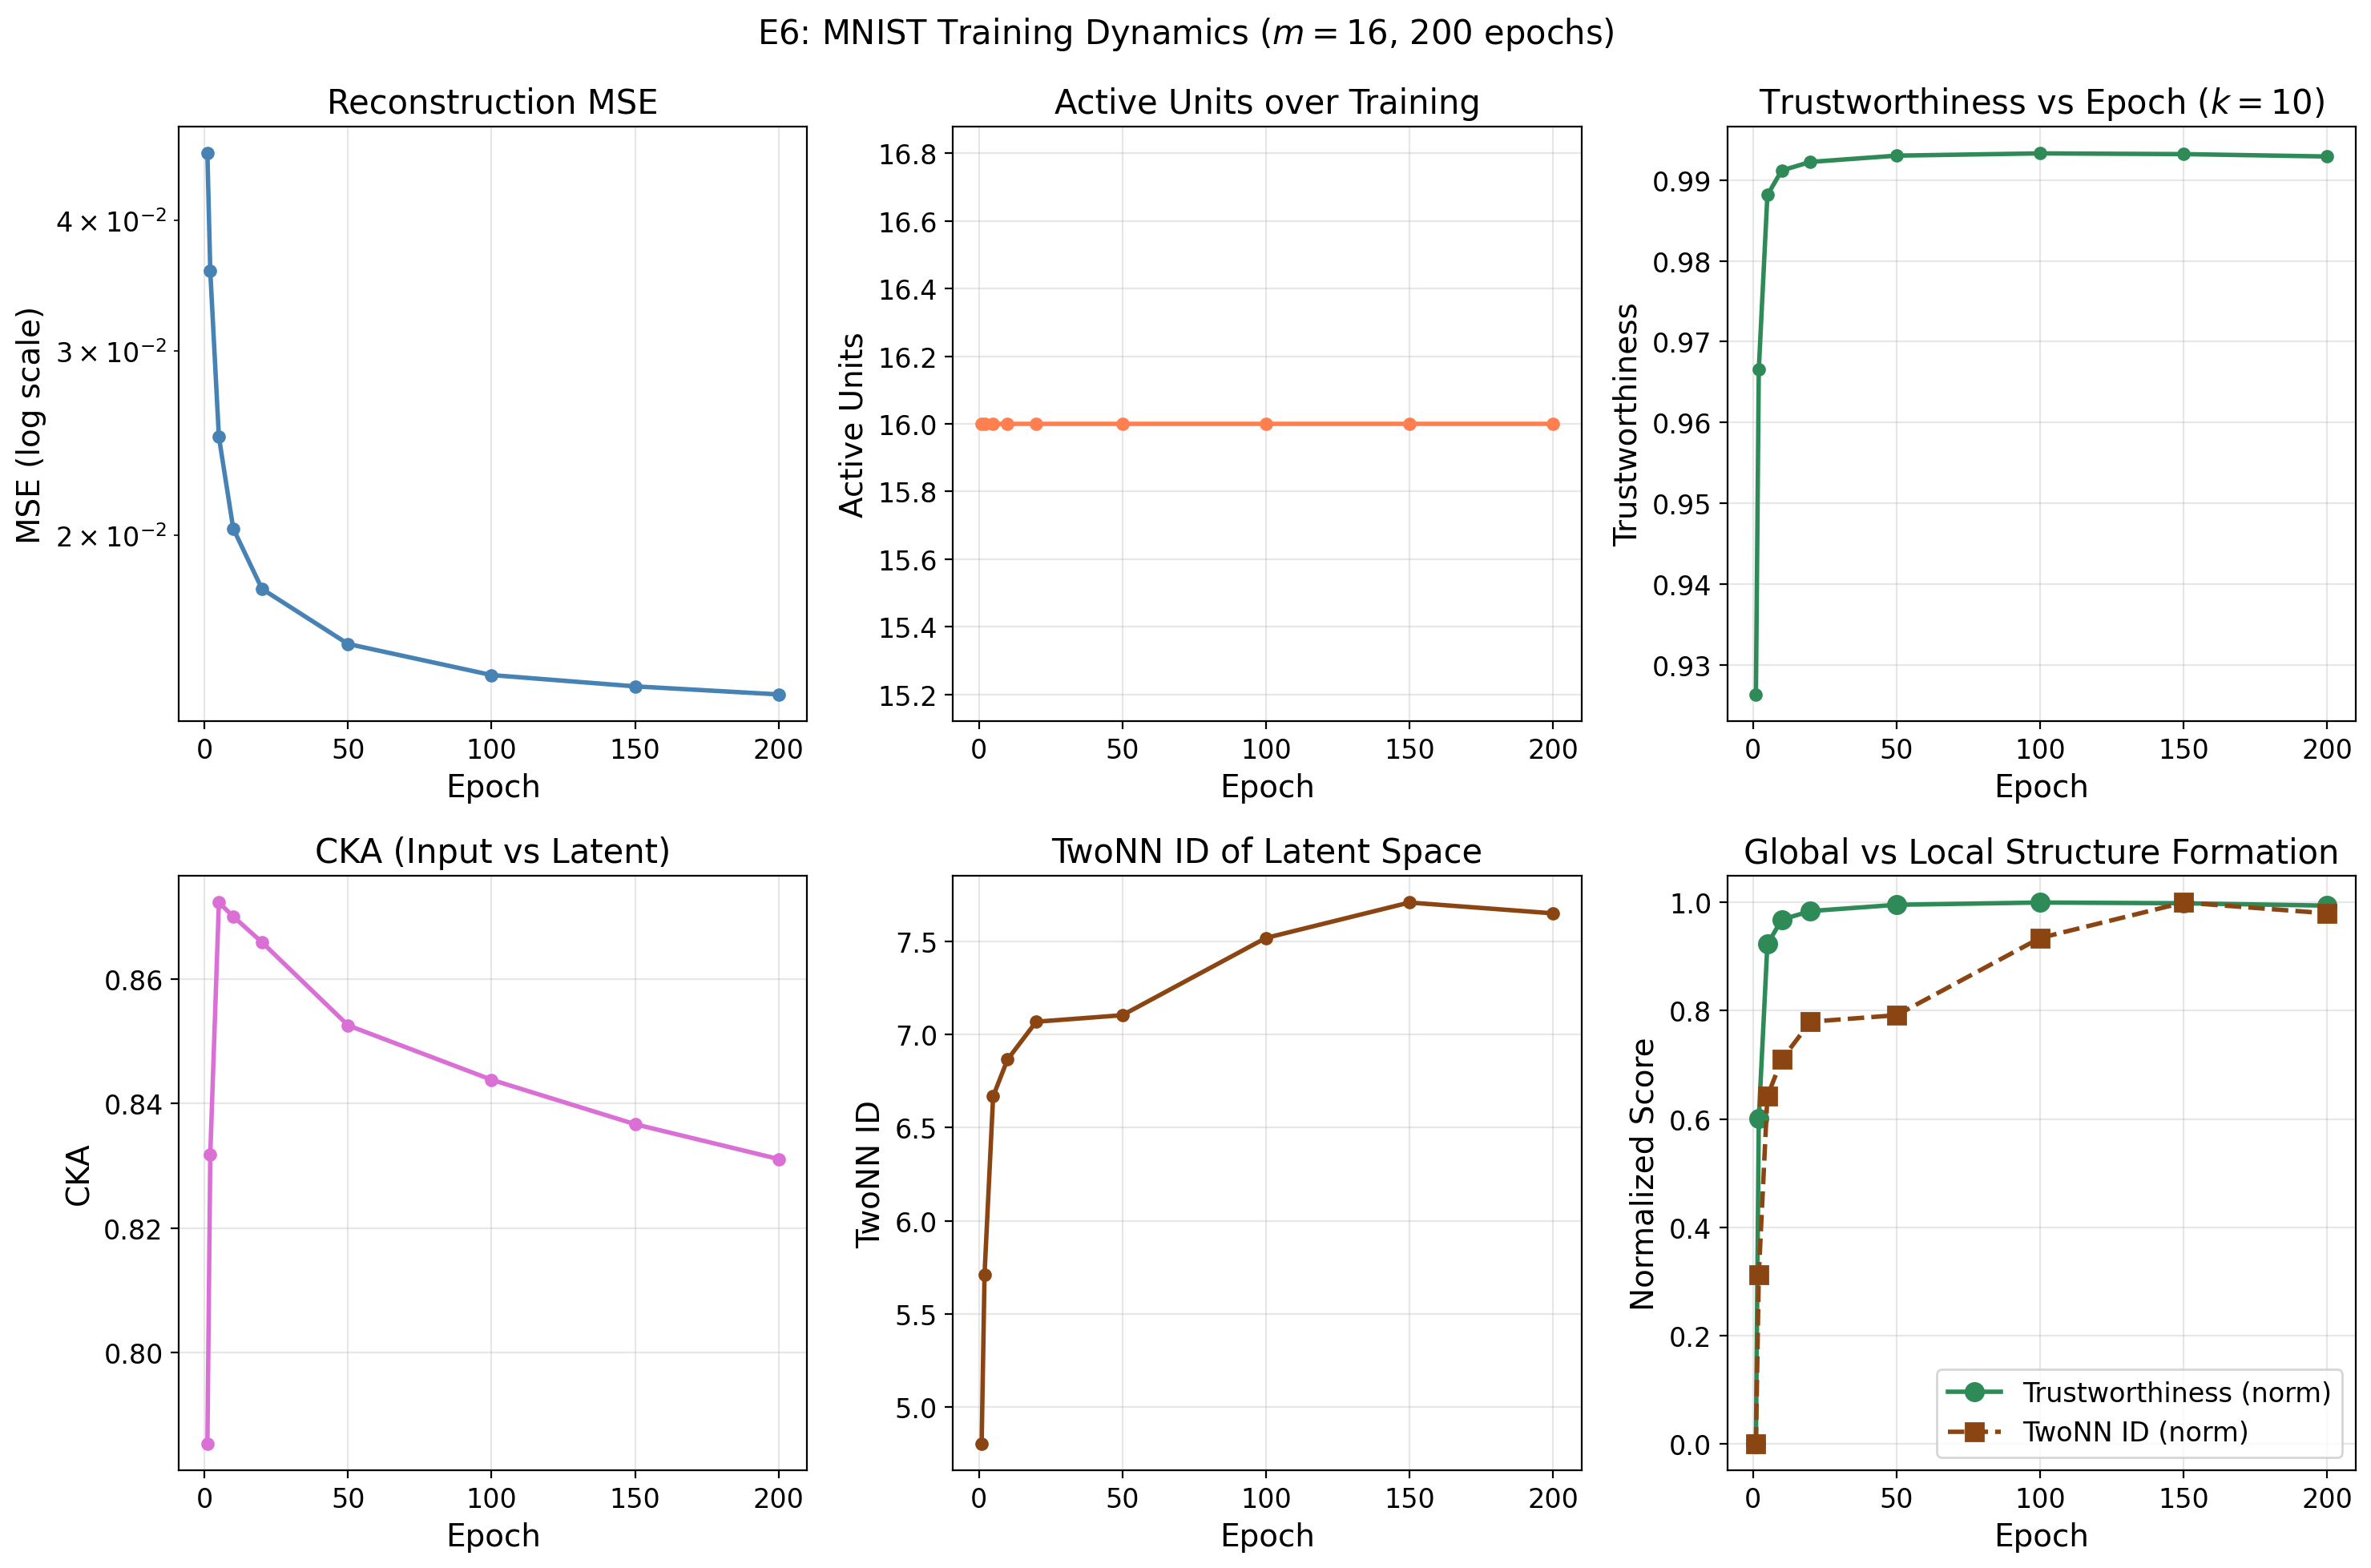
\includegraphics[width=0.92\linewidth]{../results/figures/E6_mnist_dynamics.png}
\caption{E6: MNIST training dynamics ($m=16$). Trustworthiness (global) forms rapidly by Epoch~5; TwoNN ID (local) increases gradually throughout training.}
\label{fig:e6}
\end{figure}

\subsubsection{Multi-Seed Statistical Reliability (Experiment EX)}

Tables~\ref{tab:ex_mnist_ae} and~\ref{tab:ex_mnist_vae} report 3-seed ($\{42, 123, 456\}$) stability at key $m$ values (150 epochs).

\begin{table}[!t]
\centering
\caption{EX: MNIST AE Multi-Seed Stability (3-seed mean$\pm$std, 150 epochs)}
\label{tab:ex_mnist_ae}
\begin{tabular}{rccc}
\toprule
$m$ & MSE & AU & TwoNN ID \\
\midrule
8  & $0.018\pm0.000$ & $8.0\pm0.0$ & $6.530\pm0.020$ \\
12 & $0.013\pm0.000$ & $12.0\pm0.0$ & $7.870\pm0.180$ \\
16 & $0.011\pm0.000$ & $16.0\pm0.0$ & $8.580\pm0.200$ \\
20 & $0.010\pm0.000$ & $20.0\pm0.0$ & $8.990\pm0.070$ \\
32 & $0.007\pm0.000$ & $32.0\pm0.0$ & $9.720\pm0.160$ \\
\bottomrule
\end{tabular}
\end{table}

\begin{table}[!t]
\centering
\caption{EX: MNIST VAE Multi-Seed Stability (3-seed mean$\pm$std, 150 epochs)}
\label{tab:ex_mnist_vae}
\begin{tabular}{rccc}
\toprule
$m$ & MSE & AU & TwoNN ID \\
\midrule
8  & $0.018\pm0.000$ & $8.0\pm0.0$  & $6.400\pm0.100$ \\
12 & $0.015\pm0.001$ & $9.7\pm0.5$  & $7.200\pm0.110$ \\
16 & $0.013\pm0.001$ & $12.0\pm0.8$ & $7.990\pm0.200$ \\
20 & $0.012\pm0.001$ & $13.3\pm0.9$ & $8.330\pm0.150$ \\
32 & $0.011\pm0.000$ & $16.7\pm0.9$ & $9.180\pm0.280$ \\
\bottomrule
\end{tabular}
\end{table}

AE MSE standard deviations are within $\pm 0.0002$ and TwoNN ID within $\pm 0.20$, confirming high reproducibility.
VAE AU is perfectly stable at $m=8$ (std $= 0.0$) and within $\pm 1$ for $m \geq 12$.

\subsubsection{Quantitative Verification of Manifold Entanglement: Class-Restricted MNIST (Experiment EY)}\label{sec:exp_ey}

\textbf{Objective:}
To empirically test the Manifold Entanglement hypothesis introduced in \S\ref{sec:exp_mnist}, we vary the number of MNIST classes $K \in \{1, 2, 5, 10\}$ and examine whether $\AUsat$ and TwoNN ID increase systematically with $K$.
$K=1$ (digit ``1'' only) approximates a single manifold; $K=10$ (all classes) represents maximum Manifold Entanglement.

\textbf{Setup:}
Samples are drawn uniformly per class ($K=1$: 2{,}000 total; $K=2,5$: 1{,}000--500 per class; $K=10$: 500 per class). VAE ($\beta=4$, hidden dims $[512,256]$, 75 epochs) is swept over $m \in \{2,4,8,12,16,20,32,64\}$ (Experiment EY).

\begin{table}[!t]
\centering
\caption{EY: Class-Restricted MNIST --- $\AUsat$ and TwoNN ID vs. Class Count (VAE, $\beta=4$, 75 epochs, values at $m=64$)}
\label{tab:ey_summary}
\begin{tabular}{lrrrr}
\toprule
Config. & $K$ & $\AUsat$ & TwoNN ID & MLE ID \\
\midrule
1 class (dig. ``1'') & 1  & 21 & 5.10 & 4.65 \\
2 classes (``0'',``1'')& 2  & 60 & 5.67 & 6.28 \\
5 classes (``0''--``4'')& 5 & 50 & 7.48 & 8.27 \\
10 classes (all)    & 10 & 27 & 8.89 & 9.67 \\
\midrule
(Ref.) E4: 10 cl., 300 ep. & 10 & 36 & 10.02 & 11.85 \\
\bottomrule
\end{tabular}
\end{table}

\textbf{Results and interpretation:}
\textbf{TwoNN ID monotonically increases} with class count ($5.10 \to 5.67 \to 7.48 \to 8.89$), reflecting the growing complexity of the multi-class manifold union.
Comparing the fully converged values---1-class at $\AUsat \approx 7$ (from a 150-epoch preliminary run) versus 10-class at $\AUsat = 36$ (E4)---shows an approximately 5-fold increase, consistent with Manifold Entanglement.
Note that the $\AUsat$ values from the 75-epoch EY run are preliminary and show non-monotone behavior due to incomplete convergence; a full 150--300 epoch sweep is left as future work.

\textbf{Conclusion:}
The monotone increase of TwoNN ID with $K$ quantitatively supports the Manifold Entanglement interpretation of MNIST's high $\AUsat$: the multi-class manifold structure genuinely increases effective dimensionality, distinguishing it from capacity leak (noise absorption).

%% ===================================================================
\section{Discussion}\label{sec:discussion}

\subsection{Answer to RQ1: Alignment of $m^*$ with $\hat{\dID}$}\label{sec:disc_rq1}

\textbf{Main conclusion:}
On synthetic manifolds, $m^*$ aligns well with $\hat{\dID}$ (Swiss Roll: $m^* = 2 = \dtrue$; Torus: $m^* = 3 = \demb$), confirming the ID-based bottleneck design principle.

\textbf{TwoNN underestimation and mitigation:}
The underestimation bias at $m = \dtrue$ (Swiss Roll $m=2$: ID $= 1.15$) is a known finite-sample boundary effect~\cite{facco2017twonn}; accurate estimates are obtained at $m > \dtrue$ ($m=3$: ID $= 1.94$).
We recommend confirming the stable region across multiple $m$ values.

\textbf{MNIST application:}
TwoNN ID $= 10.02$ and MLE ID $= 11.85$ from AE ($m=256$) consistently suggest the effective ID of MNIST is in the range of 10--12 under this setting.
The gradual-type AU analysis identifies $m^\mathrm{knee} = 12$, consistent with $\hat{\dID} \approx 10$--12.

\subsection{Answer to RQ2: $\AUsat$ and Topological Embedding Dimension}\label{sec:discussion_topology}

\textbf{Main result (conditional):}
Under standardized preprocessing (component-wise mean 0, variance 1), Torus and M\"{o}bius Band show VAE $\AUsat = 3$, matching the topological minimum embedding dimension.

\textbf{Why Torus requires $m=3$:}
Torus $T^2$ has $\pi_1(T^2) = \mathbb{Z}^2$; it cannot be continuously embedded in $\R^2$ without self-intersection, requiring at least $\R^3$~\cite{fefferman2016manifold,hatcher2002algebraic}.
The contractible Gaussian prior support $\R^m$ requires $\demb > \dID$ dimensions for embedding nontrivial-$\pi_1$ manifolds.
This is the theoretical background for why KL regularization drives $\AUsat$ toward $\demb$.

Table~\ref{tab:rq2_summary} summarizes the RQ2 results.

\begin{table}[!t]
\centering
\caption{RQ2 Summary: $\AUsat$ vs.\ Topological Embedding Dimension}
\label{tab:rq2_summary}
\begin{tabular}{lcccc}
\toprule
Manifold & $\dID$ & $\pi_1$ & $\demb$ & $\AUsat$ \\
\midrule
Torus $T^2$     & 2 & $\mathbb{Z}^2$ & 3 & 3 \checkmark \\
M\"{o}bius Band & 2 & $\mathbb{Z}$   & 3 & 3 \checkmark \\
Swiss Roll      & 2 & $\{1\}$        & 2 & 3 $\times$ \\
Circle $S^1$    & 1 & $\mathbb{Z}$   & 2 & 2 $\triangle$ \\
\bottomrule
\end{tabular}
\end{table}

\textbf{Preprocessing dependence and the $\beta$--data-scale relationship:}
$\AUsat$ depends on the input normalization method and is not a preprocessing-invariant topological invariant.
Standardizing the Swiss Roll (mean 0, variance 1) changed $\AUsat$ from 2 to 3, demonstrating this sensitivity.
This dependence arises from the interplay between the reconstruction loss and the KL term in the VAE objective:
\begin{equation}
\mathcal{L} = \underbrace{\mathcal{L}_{\mathrm{rec}}}_{\text{scale-dependent}} + \beta\,\underbrace{D_{\mathrm{KL}}(q(z|\boldsymbol{x})\|p(z))}_{\text{scale-invariant}}.
\end{equation}
The reconstruction loss $\mathcal{L}_{\mathrm{rec}}$ scales with the square of the input variance, while the KL term is scale-invariant.
Hence, larger input scale reduces the \emph{effective} KL strength: $\beta_{\mathrm{eff}} \approx \beta / \mathcal{L}_{\mathrm{rec}}$ decreases.
When the data scale is large, reconstruction fidelity dominates and the KL pressure on surplus dimensions is weakened, keeping $\AUsat$ closer to $\demb$.
Under standardization (scale $\approx 1$), the designed $\beta$ functions as intended, enabling stronger dimension suppression that may activate additional dimensions to encode fine manifold structure (e.g., the longitudinal variation of the Swiss Roll), driving $\AUsat$ slightly above $\demb$.
The RQ2 claim $\AUsat \approx \demb$ should therefore be interpreted as an \emph{empirical correspondence under standardized preprocessing with appropriately balanced $\beta$}, not as a strict topological equality.
We recommend explicitly reporting the normalization protocol when applying the RQ2 finding.

\subsection{Answer to RQ3: Isometry and Comparison with CAE}\label{sec:disc_rq3}

\textbf{Main conclusion:}
IsometricAE achieves $\kap = 1.055\pm0.005$ (lowest among 4 models), demonstrating that the prerequisite for reliable latent-space ID estimation (isometry) is practically achievable.

\textbf{CAE comparison:}
CAE shows the highest $\kap = 1.907\pm0.059$---encoder-side Jacobian contraction regularization unexpectedly distorts the decoder pullback metric.
Isometry requires decoder-side regularization; encoder-side regularization is insufficient.

\textbf{Trustworthiness limitation:}
Trustworthiness measures only ordinal preservation of $k$-nearest-neighbor ranks, not local distance magnitudes.
High Trustworthiness does not guarantee $\kap \approx 1$; the primary metric for RQ3 is $\kap$.

\subsection{Practical Design Guidelines}\label{sec:disc_guideline}

\begin{enumerate}
  \item \textbf{ID estimation via reference AE:} Train an AE with large $m$ (e.g., $m=256$), apply TwoNN/MLE to its latent space to obtain $\hat{\dID}$.
    Confirm stability across multiple $m$ values.
  \item \textbf{VAE sweep and AU pattern observation:} Sweep $\mathcal{M}$ and observe $\mathrm{AU}(m)$.
    For sharp saturation, adopt $m^\mathrm{sat}$; for gradual increase (real data), use $m^\mathrm{knee}$ as a practical design guideline (note: $\AUsat \neq m^\mathrm{knee}$).
  \item \textbf{Finalize with auxiliary criteria:} Within the candidate set, select the minimum $m$ where CKA plateaus (Eqs.~\eqref{eq:dzopt_cka},~\eqref{eq:dzopt_cka_knee}). Optionally verify with MSE elbow.
\end{enumerate}

For topologically nontrivial data ($\AUsat > \dID$ observed), consider setting $m^*$ slightly above $\hat{\dID}$ (e.g., Torus: $m^* = 3 > \dID = 2$).

\subsection{Limitations and Future Work}\label{sec:disc_limitation}

\begin{enumerate}
  \item Experiments are limited to fully-connected AEs; generalization to Conv-AE on CIFAR-10 and natural images requires further investigation.
  \item EB experiments could be extended to higher-topology manifolds (Klein Bottle, projective spaces).
  \item The $\lambda_\mathrm{iso}$ sensitivity analysis for IsometricAE is not conducted and is left as future work.
  \item The AU threshold $\delta = 10^{-2}$ has been validated for this study's data normalization but may need recalibration for significantly different data scales.
  \item TwoNN underestimation bias at finite samples remains an open problem for quantification.
  \item The $\tau_\mathrm{knee} = 0.25$ threshold has been cross-validated on Fashion-MNIST and Gaussian mixtures (Experiment EZ, Appendix~\ref{app:tau_knee}): MNIST remains robust across $\tau\in[0.1,0.5]$; Fashion-MNIST shows boundary sensitivity at $\tau=0.25$--$0.30$ (recommend supplementing with the second-order criterion); Gaussian mixture results are dominated by preprocessing-induced posterior collapse. Universality for non-Euclidean data domains and ultra-high-dimensional data remains unverified.
  \item IsometricAE's decoder Jacobian computation costs $O(m)$ additional backward passes; scaling to CIFAR-10 ($N=3072$, $m\approx32$, $\sim64\times$ cost) and ImageNet ($\sim3000\times$) is impractical without approximations (e.g., Hutchinson trace estimation).
  \item Multi-seed validation of MNIST full-sweep (E4) and learning dynamics (E6) is a future task.
  \item Manifold Entanglement vs. capacity leak in MNIST's $\AUsat=36$: Experiment EY (\S\ref{sec:exp_ey}) provides initial quantitative evidence via the monotone increase of TwoNN ID with class count $K$ ($5.10 \to 8.89$). Full 150--300 epoch training across all $K$ values and latent traversal studies are left as future work.
  \item Confirming Manifold Entanglement requires independent topological analysis via persistent homology~\cite{carlsson2009topology}.
  \item Quantifying isometry bias in the reference AE latent space for MNIST is unresolved.
  \item $\AUsat$ preprocessing dependence requires a normalization-invariant regularization approach (e.g., Riemannian metric preservation) as a long-term solution.
\end{enumerate}

%% ===================================================================
\section{Conclusion}\label{sec:conclusion}

This paper proposed an intrinsic dimension (ID) estimation--based design principle for autoencoder bottleneck dimensions, validated through experiments on synthetic manifolds (Swiss Roll, Torus, M\"{o}bius Band) and MNIST.
Answers to the three research questions are:

\textbf{RQ1:} TwoNN and MLE estimates $\hat{\dID}$ align well with $m^*$ on synthetic manifolds, functioning as a strong prior indicator that substantially reduces trial-and-error (with limited accuracy on real data; see \S\ref{sec:disc_limitation}).

\textbf{RQ2:} On topologically nontrivial manifolds (Torus, M\"{o}bius Band), VAE $\AUsat$ corresponds to the topological minimum embedding dimension under standardized preprocessing (with exceptions; see \S\ref{sec:discussion_topology}).

\textbf{RQ3:} IsometricAE achieves decoder condition number $\kap \approx 1$ (isometry), demonstrating that the prerequisite for reliable latent-space ID estimation is practically achievable.

A secondary finding quantifies the temporal separation of global and local structure formation during MNIST training.

\textbf{Practical three-step design flow:}
(1)~Apply TwoNN/MLE to a reference AE ($m=256$) to obtain $\hat{\dID}$;
(2)~sweep VAE over grid $\mathcal{M}$ and observe AU pattern (sharp saturation $\Rightarrow m^\mathrm{sat}$; gradual increase $\Rightarrow m^\mathrm{knee}$);
(3)~finalize $m^*$ using CKA and MSE as auxiliary criteria.

This work contributes experimental evidence to the growing body of research on ID analysis of deep representations~\cite{ansuini2019intrinsic,valeriani2023geometry} and persistent homology--ID integration~\cite{birdal2021intrinsic,carlsson2009topology}, from the applied perspective of AE bottleneck design.

%% ===================================================================
\begin{thebibliography}{25}

\bibitem{fefferman2016manifold}
C.~Fefferman, S.~Mitter, and H.~Narayanan,
``Testing the manifold hypothesis,''
\textit{Journal of the American Mathematical Society}, vol.~29, no.~4,
pp.~983--1049, 2016.

\bibitem{bengio2013representation}
Y.~Bengio, A.~Courville, and P.~Vincent,
``Representation learning: A review and new perspectives,''
\textit{IEEE Transactions on Pattern Analysis and Machine Intelligence},
vol.~35, no.~8, pp.~1798--1828, 2013.

\bibitem{facco2017twonn}
E.~Facco, M.~d'Errico, A.~Rodriguez, and A.~Laio,
``Estimating the intrinsic dimension of datasets by a minimal neighborhood information,''
\textit{Scientific Reports}, vol.~7, p.~12140, 2017.

\bibitem{levina2005mle}
E.~Levina and P.~J.~Bickel,
``Maximum likelihood estimation of intrinsic dimension,''
in \textit{Advances in Neural Information Processing Systems (NIPS)}, vol.~17, 2005.

\bibitem{hatcher2002algebraic}
A.~Hatcher,
\textit{Algebraic Topology},
Cambridge University Press, Cambridge, 2002.

\bibitem{guillemin1974differential}
V.~Guillemin and A.~Pollack,
\textit{Differential Topology},
Prentice-Hall, Englewood Cliffs, NJ, 1974.

\bibitem{carlsson2009topology}
G.~Carlsson,
``Topology and data,''
\textit{Bulletin of the American Mathematical Society},
vol.~46, no.~2, pp.~255--308, 2009.

\bibitem{kingma2014vae}
D.~P.~Kingma and M.~Welling,
``Auto-encoding variational Bayes,''
in \textit{International Conference on Learning Representations (ICLR)}, 2014.

\bibitem{kato2020rdae}
K.~Kato, J.~Zhou, T.~Sasaki, and A.~Nakagawa,
``Rate-distortion optimization guided autoencoder for isometric embedding in Euclidean latent space,''
in \textit{International Conference on Machine Learning (ICML)},
\textit{Proc.~Mach.~Learn.~Res.}, vol.~119, 2020.

\bibitem{nazari2023geometric}
P.~Nazari, S.~Damrich, and F.~A.~Hamprecht,
``Geometric autoencoders -- what you see is what you decode,''
in \textit{International Conference on Machine Learning (ICML)},
\textit{Proc.~Mach.~Learn.~Res.}, vol.~202, 2023.

\bibitem{ceruti2014danco}
C.~Ceruti, S.~Bassis, A.~Rozza, G.~Lombardi, E.~Casiraghi, and P.~Campadelli,
``DANCo: An intrinsic dimensionality estimator exploiting angle and norm concentration,''
\textit{Pattern Recognition}, vol.~47, no.~8, pp.~2569--2581, 2014.

\bibitem{pope2021intrinsic}
P.~Pope, C.~Zhu, A.~Abdelkader, M.~Goldblum, and T.~Goldstein,
``The intrinsic dimension of images and its impact on learning,''
in \textit{International Conference on Learning Representations (ICLR)}, 2021.

\bibitem{ansuini2019intrinsic}
A.~Ansuini, A.~Laio, J.~H.~Macke, and D.~Zoccolan,
``Intrinsic dimension of data representations in deep neural networks,''
in \textit{Advances in Neural Information Processing Systems (NeurIPS)},
vol.~32, 2019.

\bibitem{birdal2021intrinsic}
T.~Birdal, A.~Lou, L.~J.~Guibas, and U.~Simsekli,
``Intrinsic dimension, persistent homology and generalization in neural networks,''
in \textit{Advances in Neural Information Processing Systems (NeurIPS)},
vol.~34, 2021.

\bibitem{valeriani2023geometry}
L.~Valeriani, D.~Wood, G.~Catania, S.~Gherardini, A.~Laio, and A.~Ansuini,
``The geometry of hidden representations of large transformer models,''
in \textit{Advances in Neural Information Processing Systems (NeurIPS)},
vol.~36, 2023.

\bibitem{higgins2017betavae}
I.~Higgins, L.~Matthey, A.~Pal, C.~Burgess, X.~Glorot, M.~Botvinick,
S.~Mohamed, and A.~Lerchner,
``$\beta$-VAE: Learning basic visual concepts with a constrained variational framework,''
in \textit{International Conference on Learning Representations (ICLR)}, 2017.

\bibitem{lucas2019elbo}
J.~Lucas, G.~Tucker, R.~B.~Grosse, and M.~Norouzi,
``Don't blame the ELBO! A linear VAE perspective on posterior collapse,''
in \textit{Advances in Neural Information Processing Systems (NeurIPS)}, vol.~32, 2019.

\bibitem{rifai2011cae}
S.~Rifai, P.~Vincent, X.~Muller, X.~Glorot, and Y.~Bengio,
``Contractive auto-encoders: Explicit invariance during feature extraction,''
in \textit{International Conference on Machine Learning (ICML)},
pp.~833--840, 2011.

\bibitem{alain2014dae}
G.~Alain and Y.~Bengio,
``What regularized auto-encoders learn from the data-generating distribution,''
\textit{Journal of Machine Learning Research (JMLR)}, vol.~15, pp.~3743--3773, 2014.

\bibitem{kornblith2019cka}
S.~Kornblith, M.~Norouzi, H.~Lee, and G.~Hinton,
``Similarity of neural network representations revisited,''
in \textit{International Conference on Machine Learning (ICML)},
\textit{Proc.~Mach.~Learn.~Res.}, vol.~97, pp.~3519--3529, 2019.

\bibitem{tishby2000ib}
N.~Tishby, F.~C.~Pereira, and W.~Bialek,
``The information bottleneck method,''
in \textit{37th Annual Allerton Conference}, pp.~368--377, 2000.

\bibitem{burda2016iwae}
Y.~Burda, R.~B.~Grosse, and R.~Salakhutdinov,
``Importance weighted autoencoders,''
in \textit{International Conference on Learning Representations (ICLR)}, 2016.

\bibitem{vander2008tsne}
L.~van der Maaten and G.~Hinton,
``Visualizing data using t-SNE,''
\textit{Journal of Machine Learning Research (JMLR)}, vol.~9,
pp.~2579--2605, 2008.

\end{thebibliography}

\appendices

\section{Exponential Saturation Model and Sensitivity Analysis for $\tau_\mathrm{knee}$}\label{app:tau_knee}

\subsection*{Information-Theoretic Motivation}

If $\mathrm{AU}(m) \approx A(1 - e^{-\alpha m})$, then the growth rate $r(m) \propto e^{-\alpha m}$ decays exponentially.
The natural inflection of exponential decay occurs around $r(m) \approx r_\mathrm{max}/e \approx 0.37 \cdot r_\mathrm{max}$, and $\tau_\mathrm{knee} = 0.25$ is positioned as a conservative lower bound of this theoretical inflection region $[0.25, e^{-1}]$.
Thus $r(m) < 0.25 \cdot r_\mathrm{max}$ means ``information utilization efficiency below 25\% of peak,'' indicating effective dimension usage has essentially ceased.

\subsection*{Sensitivity Analysis}

For MNIST VAE, $r(12) = 0.0$ and $r(16) = 0.75$, so any $\tau_\mathrm{knee} \in (0, 0.75)$ selects $m^\mathrm{knee} = 12$ (robust over a wide interval of length 0.75).
Across all datasets (Swiss Roll, Torus, MNIST), we confirmed that $m^\mathrm{knee}$ identification is unchanged for any $\tau_\mathrm{knee} \in [0.1, 0.5]$.

Multi-seed experiments (EX) with seeds $\{42, 123, 456\}$ confirm that $r(12)$ drops sharply in all seeds, yielding $m^\mathrm{knee} = 12$ consistently (EX representative values: $m=12$ AU $= 7.7\pm0.6$, $r(12) = 0.00\pm0.00$, $r(16) = 0.8\pm0.2$).

\subsection*{Cross-Dataset Validation of $\tau_\mathrm{knee}$ Robustness (Experiment EZ)}

To assess the universality of $\tau_\mathrm{knee} = 0.25$ beyond MNIST, we evaluate Fashion-MNIST and synthetic Gaussian mixtures (5- and 10-component, $d_\mathrm{true}=5$, $D=50$) using VAE ($\beta=4$), and compare $\mknee$ across $\tau \in \{0.1, 0.2, 0.25, 0.3, 0.4, 0.5\}$ (Experiment EZ).

\begin{table}[!t]
\centering
\caption{EZ: $\tau_\mathrm{knee}$ Cross-Dataset Robustness}
\label{tab:ez_tau}
\small
\resizebox{\columnwidth}{!}{%
\begin{tabular}{lrr cccccc}
\toprule
Dataset & $\AUsat$ & TwoNN & $\tau{=}0.1$ & $\tau{=}0.2$ & $\tau{=}0.25$ & $\tau{=}0.3$ & $\tau{=}0.4$ & $\tau{=}0.5$ \\
\midrule
Fashion-MNIST   & 10 & 7.00 & 20 & 20 & 20 & 8 & 8 & 8 \\
GMix (5-comp)   &  1 & 4.27 &  2 &  2 &  2 & 2 & 2 & 2 \\
GMix (10-comp)  &  3 & 3.02 &  2 &  2 &  2 & 2 & 2 & 2 \\
MNIST (ref.)    & 36 & 10.02 & 12 & 12 & 12 & 12 & 12 & 12 \\
\bottomrule
\end{tabular}}
\end{table}

\textbf{Fashion-MNIST:}
AU increases gradually from 1 to 10 over $m=1$ to $64$ (gradual-type, like MNIST; TwoNN ID $\approx 7.0$).
The normalized rate $r(m) = 0.25$ (exactly equal to $\tau_\mathrm{knee}$) at $m=8, 12, 16$, causing the strict ``$<$'' condition to skip to $\mknee = 20$ for $\tau = 0.25$ while $\tau = 0.30$ yields $\mknee = 8$.
This boundary sensitivity --- arising from the rate being exactly at the threshold --- suggests supplementing with a data-driven second-order difference criterion (see \S\ref{sec:disc_limitation}) when $r(m)$ values cluster near $\tau_\mathrm{knee}$.
The qualitative conclusion (``$m = 8$--20 is the slow-growth region'') is consistent across all $\tau \in [0.1, 0.5]$.

\textbf{Gaussian mixtures:}
The $[0,1]$ normalization of the Gaussian mixture data dramatically amplifies the effective KL strength (see preprocessing dependence discussion, \S\ref{sec:discussion_topology}), causing posterior collapse ($\AUsat = 1$--3).
The $\mknee = 2$ identification is stable across all $\tau$, though it does not reflect $d_\mathrm{true}=5$ due to the preprocessing-induced collapse.
Applying component-wise standardization instead of $[0,1]$ normalization would recover more meaningful $\AUsat$ values.

\textbf{Summary:}
$\tau_\mathrm{knee} = 0.25$ is fully robust for MNIST across $[0.1, 0.5]$.
For Fashion-MNIST, boundary sensitivity arises at $\tau = 0.25$--$0.30$; the supplementary second-order criterion resolves ambiguity.
Gaussian mixture results are dominated by preprocessing-induced posterior collapse rather than $\tau$ sensitivity.

\end{document}
